\documentclass[a4paper]{article}

\def\npart {IB}
\def\nterm {Easter}
\def\nyear {2015}
\def\nlecturer {P.\ K.\ Townsend}
\def\ncourse {Variational Principles}
\def\nofficial {http://www.damtp.cam.ac.uk/user/examples/B6La.pdf}

\usepackage{myheader}

\begin{document}
\maketitle
{\small
\noindent Stationary points for functions on $\R^n$. Necessary and sufficient conditions for minima and maxima. Importance of convexity. Variational problems with constraints; method of Lagrange multipliers. The Legendre Transform; need for convexity to ensure invertibility; illustrations from thermodynamics.\hspace*{\fill} [4]

\vspace{5pt}
\noindent The idea of a functional and a functional derivative. First variation for functionals, Euler-Lagrange equations, for both ordinary and partial differential equations. Use of Lagrange multipliers and multiplier functions.\hspace*{\fill} [3]

\vspace{5pt}
\noindent Fermat's principle; geodesics; least action principles, Lagrange's and Hamilton's equations for particles and fields. Noether theorems and first integrals, including two forms of Noether's theorem for ordinary differential equations (energy and momentum, for example). Interpretation in terms of conservation laws.\hspace*{\fill} [3]

\vspace{5pt}
\noindent Second variation for functionals; associated eigenvalue problem.\hspace*{\fill} [2]}

\tableofcontents
\setcounter{section}{-1}
\section{Introduction}
Consider a light ray travelling towards a mirror and being reflected.
\begin{center}
  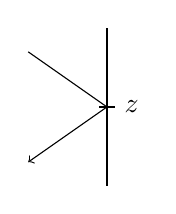
\begin{tikzpicture}
    \draw (1, 1) -- (1, -1);
    \draw (0.9, 0) -- (1.1, 0) node [right] {$z$};
    \draw [->] (0, 0.7) -- (1, 0) -- (0, -0.7);
  \end{tikzpicture}
\end{center}
We see that the light ray travels towards the mirror, gets reflected at $z$, and hits the (invisible) eye. What determines the path taken? The usual answer would be that the reflected angle shall be the same as the incident angle. However, ancient Greek mathematician Hero of Alexandria provided a different answer: the path of the light minimizes the total distance travelled.

We can assume that light travels in a straight line except when reflected. Then we can characterize the path by a single variable $z$, the point where the light ray hits the mirror. Then we let $L(z)$ to be the length of the path, and we can solve for $z$ by setting $L'(z) = 0$.

This principle sounds reasonable - in the absence of mirrors, light travels in a straight line - which is the shortest path between two points. But is it always true that the \emph{shortest} path is taken? No! We only considered a plane mirror, and this doesn't hold if we have, say, a spherical mirror. However, it turns out that in all cases, the path is a stationary point of the length function, i.e.\ $L'(z) = 0$.

Fermat put this principle further. Assuming that light travels at a finite speed, the shortest path is the path that takes the minimum time. Fermat's principle thus states that
\begin{center}
  Light travels on the path that takes the shortest time.
\end{center}
This alternative formulation has the advantage that it applies to refraction as well. Light travels at different speeds in different mediums. Hence when they travel between mediums, they will change direction such that the total time taken is minimized.

We usually define the refractive index $n$ of a medium to be $n = 1/v$, where $v$ is the velocity of light in the medium. Then we can write the variational principle as
\begin{center}
  minimize $\displaystyle \int_{\text{path}} n\;\d s$,
\end{center}
where $\d s$ is the path length element. This is easy to solve if we have two distinct mediums. Since light travels in a straight line in each medium, we can simply characterize the path by the point where the light crosses the boundary. However, in the general case, we should be considering \emph{any} possible path between two points. In this case, we could no longer use ordinary calculus, and need new tools - calculus of variations.

In calculus of variations, the main objective is to find a function $x(t)$ that minimizes an integral $\int f(x)\;\d t$ for some function $f$. For example, we might want to minimize $\int (x^2 + x)\;\d t$. This differs greatly from ordinary minimization problems. In ordinary calculus, we minimize a function $f(x)$ for all possible values of $x\in \R$. However, in calculus of variations, we will be minimizing the integral $\int f(x)\;\d t$ over all possible \emph{functions} $x(t)$.

\section{Multivariate calculus}
Before we start calculus of variations, we will first have a brief overview of minimization problems in ordinary calculus. Unless otherwise specified, $f$ will be a function $\R^n \to \R$. For convenience, we write the argument of $f$ as $\mathbf{x} = (x_1, \cdots, x_n)$ and $x = |\mathbf{x}|$. We will also assume that $f$ is sufficiently smooth for our purposes.

\subsection{Stationary points}
The quest of minimization starts with finding stationary points.
\begin{defi}[Stationary points]
  \emph{Stationary points} are points in $\R^n$ for which $\nabla f = \mathbf{0}$, i.e.
  \[
    \frac{\partial f}{\partial x_1} = \frac{\partial f}{\partial x_2} = \cdots = \frac{\partial f}{\partial x_n} = 0
  \]
\end{defi}
All minima and maxima are stationary points, but knowing that a point is stationary is not sufficient to determine which type it is. To know more about the nature of a stationary point, we Taylor expand $f$ about such a point, which we assume is $\mathbf{0}$ for notational convenience.
\begin{align*}
  f(\mathbf{x}) &= f(\mathbf{0}) + \mathbf{x}\cdot \nabla f + \frac{1}{2}\sum_{i, j}x_ix_j\frac{\partial^2 f}{\partial x_i \partial x_j} + O(x^3).\\
  &= f(\mathbf{0}) + \frac{1}{2}\sum_{i, j}x_ix_j\frac{\partial^2 f}{\partial x_i \partial x_j} + O(x^3).
\end{align*}
The second term is so important that we have a name for it:
\begin{defi}[Hessian matrix]
  The \emph{Hessian matrix} is
  \[
    H_{ij}(\mathbf{x}) = \frac{\partial^2 f}{\partial x_i \partial x_j}
  \]
\end{defi}
Using summation notation, we can write our result as
\[
  f(\mathbf{x}) - f(\mathbf{0}) = \frac{1}{2}x_i H_{ij}x_j + O(x^3).
\]
Since $H$ is symmetric, it is diagonalizable. Thus after rotating our axes to a suitable coordinate system, we have
\[
  H_{ij}' =
  \begin{pmatrix}
    \lambda_1 & 0 & \cdots & 0\\
    0 & \lambda_2 & \cdots & 0\\
    \vdots & \vdots & \ddots & \vdots \\
    0 & 0 & \cdots & \lambda_n
  \end{pmatrix},
\]
where $\lambda_i$ are the eigenvalues of $H$. Since $H$ is real symmetric, these are all real. In our new coordinate system, we have
\[
  f(\mathbf{x}) - f(\mathbf{0}) = \frac{1}{2}\sum_{i = 1}^n \lambda_i (x_i')^2
\]
This is useful information. If all eigenvalues $\lambda_i$ are positive, then $f(\mathbf{x}) - f(\mathbf{0})$ must be positive (for small $\mathbf{x}$). Hence our stationary point is a local minimum. Similarly, if all eigenvalues are negative, then it is a local maximum.

If there are mixed signs, say $\lambda_1 > 0$ and $\lambda_2 < 0$, then $f$ increases in the $x_1$ direction and decreases in the $x_2$ direction. In this case we say we have a saddle point.

If some $\lambda = 0$, then we have a \emph{degenerate stationary point}. To identify the nature of this point, we must look at even higher derivatives.

In the special case where $n = 2$, we do not need to explicitly find the eigenvalues. We know that $\det H$ is the product of the two eigenvalues. Hence if $\det H$ is negative, the eigenvalues have different signs, and we have a saddle. If $\det H$ is positive, then the eigenvalues are of the same sign.

To determine if it is a maximum or minimum, we can look at the trace of $H$, which is the sum of eigenvalues. If $\tr H$ is positive, then we have a local minimum. Otherwise, it is a local maximum.

\begin{eg}
  Let $f(x, y) = x^3 + y^3 - 3xy$. Then
  \[
    \nabla f = 3(x^2 - y, y^2 - x).
  \]
  This is zero iff $x^2 = y$ and $y^2 = x$. This is satisfied iff $y^4 = y$. So either $y = 0$, or $y = 1$. So there are two stationary points: $(0, 0)$ and $(1, 1)$.

  The Hessian matrix is
  \[
    H =
    \begin{pmatrix}
      6x & -3\\
      -3 & 6y
    \end{pmatrix},
  \]
  and we have
  \begin{align*}
    \det H &= 9(4xy - 1)\\
    \tr H &= 6(x + y).
  \end{align*}
  At $(0, 0)$, $\det H < 0$. So this is a saddle point. At $(1, 1)$, $\det H > 0$, $\tr H > 0$. So this is a local minimum.
\end{eg}
\subsection{Convex functions}
\subsubsection{Convexity}
\emph{Convex functions} is an important class of functions that has a lot of nice properties. For example, stationary points of convex functions are all minima, and a convex function can have at most one minimum value. To define convex functions, we need to first define a \emph{convex set}.

\begin{defi}[Convex set]
  A set $S\subseteq \R^n$ is \emph{convex} if for any distinct $\mathbf{x}, \mathbf{y}\in S, t\in (0, 1)$, we have $(1 - t)\mathbf{x} + t\mathbf{y} \in S$. Alternatively, any line joining two points in $S$ lies completely within $S$.
  \begin{center}
    \begin{tikzpicture}
      \begin{scope}[shift={(-2, 0)}]
        \draw [fill=gray!50!white] plot [smooth cycle, tension=0.7] coordinates {(0, 1) (-0.7, 0.7) (-1, 0) (-0.6, -1) (0, 0) (0.6, -1) (1, 0) (0.7, 0.7)};
        \draw (-0.5, -0.5) node [circ] {} -- (0.5, -0.5) node [circ] {};

        \node at (0, -1.5) {non-convex};
      \end{scope}

      \begin{scope}[shift={(2, 0)}]
        \draw [fill=gray!50!white] plot [smooth cycle, tension=0.7] coordinates {(0, 1) (-0.7, 0.7) (-1, 0) (-0.6, -1) (0.6, -1) (1, 0) (0.7, 0.7)};
        \node at (0, -1.5) {convex};
      \end{scope}
    \end{tikzpicture}
  \end{center}
\end{defi}

\begin{defi}[Convex function]
  A function $f: \R^n \to \R$ is \emph{convex} if
  \begin{enumerate}
    \item The domain $D(f)$ is convex
    \item The function $f$ lies below (or on) all its chords, i.e.
      \[
        f((1 - t)\mathbf{x} + t\mathbf{y}) \leq (1 - t)f(\mathbf{x}) + tf(\mathbf{y}) \tag{$*$}
      \]
      for all $\mathbf{x}, \mathbf{y}\in D(f), t\in (0, 1)$.
  \end{enumerate}
  A function is \emph{strictly convex} if the inequality is strict, i.e.
  \[
    f((1 - t)\mathbf{x} + t\mathbf{y}) < (1 - t)f(\mathbf{x}) + tf(\mathbf{y}).
  \]
  \begin{center}
    \begin{tikzpicture}
      \draw(-2, 4) -- (-2, 0) -- (2, 0) -- (2, 4);
      \draw (-1.3, 0.1) -- (-1.3, -0.1) node [below] {$x$};
      \draw (1.3, 0.1) -- (1.3, -0.1) node [below] {$y$};
      \draw (-1.7, 2) parabola bend (-.2, 1) (1.7, 3.3);
      \draw [dashed] (-1.3, 0) -- (-1.3, 1.53) node [circ] {};
      \draw [dashed] (1.3, 0) -- (1.3, 2.42) node [circ] {};
      \draw (-1.3, 1.53) -- (1.3, 2.42);
      \draw [dashed] (0, 0) node [below] {\tiny $(1 - t)x + ty$} -- (0, 1.975) node [above] {\tiny$(1 - t)f(x) + t f(y)\quad\quad\quad\quad\quad\quad$} node [circ] {};
    \end{tikzpicture}
  \end{center}
  A function $f$ is (strictly) concave iff $-f$ is (strictly) convex.
\end{defi}

\begin{eg}\leavevmode
  \begin{enumerate}
    \item $f(x) = x^2$ is strictly convex.
    \item $f(x) = |x|$ is convex, but not strictly.
    \item $f(x) = \frac{1}{x}$ defined on $x > 0$ is strictly convex.
    \item $f(x) = \frac{1}{x}$ defined on $\R^* = \R \setminus \{0\}$ is \emph{not} convex. Apart from the fact that $\R^*$ is not a convex domain. But even if we defined, like $f(0) = 0$, it is not convex by considering the line joining $(-1, -1)$ and $(1, 1)$ (and in fact $f(x) = \frac{1}{x}$ defined on $x < 0$ is concave).
  \end{enumerate}
\end{eg}
\subsubsection{First-order convexity condition}
While the definition of a convex function seems a bit difficult to work with, if our function is differentiable, it is easy to check if it is convex.

First assume that our function is once differentiable, and we attempt to find a first-order condition for convexity. Suppose that $f$ is convex. For fixed $\mathbf{x}, \mathbf{y}$, we define the function
\[
  h(t) = (1 - t)f(\mathbf{x}) + tf(\mathbf{y}) - f((1 - t)\mathbf{x} + t \mathbf{y}).
\]
By the definition of convexity of $f$, we must have $h(t) \geq 0$. Also, trivially $h(0) = 0$. So
\[
  \frac{h(t) - h(0)}{t} \geq 0
\]
for any $t\in (0, 1)$. So
\[
  h'(0) \geq 0.
\]
On the other hand, we can also differentiate $h$ directly and evaluate at $0$:
\[
  h'(0) = f(\mathbf{y}) - f(\mathbf{x}) - (\mathbf{y} - \mathbf{x})\cdot \nabla f (\mathbf{x}).
\]
Combining our two results, we know that
\[
  f(\mathbf{y}) \geq f(\mathbf{x}) + (\mathbf{y} - \mathbf{x})\cdot \nabla f(\mathbf{x}) \tag{$\dagger$}
\]
It is also true that this condition implies convexity, which is an easy result.

How can we interpret this result? The equation $f(\mathbf{x}) + (\mathbf{y} - \mathbf{x}) \cdot \nabla f(\mathbf{x}) = 0$ defines the tangent plane of $f$ at $\mathbf{x}$. Hence this condition is saying that a convex differentiable function lies above all its tangent planes.

We immediately get the corollary
\begin{cor}
  A stationary point of a convex function is a global minimum. There can be more than one global minimum (e.g.\ a constant function), but there is at most one if the function is strictly convex.
\end{cor}

\begin{proof}
  Given $\mathbf{x}_0$ such that $\nabla f(\mathbf{x}_0) = \mathbf{0}$, $(\dagger)$ implies that for any $\mathbf{y}$,
  \[
    f(\mathbf{y}) \geq f(\mathbf{x}_0) + (\mathbf{y} - \mathbf{x}_0)\cdot \nabla f(\mathbf{x}_0) = f(\mathbf{x}_0). \qedhere
  \]
\end{proof}
We can write our first-order convexity condition in a different way. We can rewrite $(\dagger)$ into the form
\[
  (\mathbf{y} - \mathbf{x}) \cdot [\nabla f(\mathbf{y}) - \nabla f(\mathbf{x})] \geq f(\mathbf{x}) - f(\mathbf{y}) - (\mathbf{x} - \mathbf{y}) \cdot \nabla f(\mathbf{y}).
\]
By applying $(\dagger)$ to the right hand side (with $\mathbf{x}$ and $\mathbf{y}$ swapped), we know that the right hand side is $\geq 0$. So we have another first-order condition:
\[
  (\mathbf{y} - \mathbf{x})\cdot [\nabla f(\mathbf{y}) - \nabla f(\mathbf{x})] \geq 0,
\]
It can be shown that this is equivalent to the other conditions.

This condition might seem a bit weird to comprehend, but all it says is that $\nabla f(\mathbf{x})$ is a non-decreasing function. For example, when $n = 1$, the equation states that $(y - x)(f'(y) - f'(x)) \geq 0$, which is the same as saying $f'(y) \geq f'(x)$ whenever $y > x$.

\subsubsection{Second-order convexity condition}
We have an even nicer condition when the function is twice differentiable. We start with the equation we just obtained:
\[
  (\mathbf{y} - \mathbf{x})\cdot [\nabla f(\mathbf{y}) - \nabla f(\mathbf{x})] \geq 0,
\]
Write $\mathbf{y} = \mathbf{x} + \mathbf{h}$. Then
\[
  \mathbf{h} \cdot (\nabla f(\mathbf{x} + \mathbf{h}) - \nabla f(\mathbf{x})) \geq 0.
\]
Expand the left in Taylor series. Using suffix notation, this becomes
\[
  h_i [h_j \nabla_j \nabla_i f + O(h^2)] \geq 0.
\]
But $\nabla_j \nabla_i f = H_{ij}$. So we have
\[
  h_i H_{ij}h_j + O(h^3) \geq 0
\]
This is true for all $h$ if the Hessian $H$ is positive semi-definite (or simply positive), i.e.\ the eigenvalues are non-negative. If they are in fact all positive, then we say $H$ is positive definite.

Hence convexity implies that the Hessian matrix is positive for all $\mathbf{x}\in D(f)$. Strict convexity implies that it is positive definite.

The converse is also true --- if the Hessian is positive, then it is convex.

\begin{eg}
  Let $f(x, y) = \frac{1}{xy}$ for $x, y > 0$. Then the Hessian is
  \[
    H = \frac{1}{xy}
    \begin{pmatrix}
      \frac{2}{x^2} & \frac{1}{xy}\\
      \frac{1}{xy} & \frac{2}{y^2}
    \end{pmatrix}
  \]
  The determinant is
  \[
    \det H = \frac{3}{x^4y^4} > 0
  \]
  and the trace is
  \[
    \tr H = \frac{2}{xy}\left(\frac{1}{x^2} + \frac{1}{y^2}\right) > 0.
  \]
  So $f$ is convex.

  To conclude that $f$ is convex, we only used the fact that $xy$ is positive, instead of $x$ and $y$ being individually positive. Then could we relax the domain condition to be $xy > 0$ instead? The answer is no, because in this case, the function will no longer be convex!
\end{eg}

\subsection{Legendre transform}
The Legendre transform is an important tool in classical dynamics and thermodynamics. In classical dynamics, it is used to transform between the Lagrangian and the Hamiltonian. In thermodynamics, it is used to transform between the energy, Helmholtz free energy and enthalpy. Despite its importance, the definition is slightly awkward.

Suppose that we have a function $f(x)$, which we'll assume is differentiable. For some reason, we want to transform it into a function of the conjugate variable $p = \frac{\d f}{\d x}$ instead. In most applications to physics, this quantity has a particular physical significance. For example, in classical dynamics, if $L$ is the Lagrangian, then $p = \frac{\partial L}{\partial \dot{x}}$ is the (conjugate) momentum. $p$ also has a context-independent geometric interpretation, which we will explore later. For now, we will assume that $p$ is more interesting than $x$.

Unfortunately, the obvious option $f^*(p) = f(x(p))$ is not the transform we want. There are various reasons for this, but the major reason is that it is \emph{ugly}. It lacks any mathematical elegance, and has almost no nice properties at all.

In particular, we want our $f^*(p)$ to satisfy the property
\[
  \frac{\d f^*}{\d p} = x.
\]
This says that if $p$ is the conjugate of $x$, then $x$ is the conjugate of $p$. We will soon see how this is useful in the context of thermodynamics.

The symmetry is better revealed if we write in terms of differentials. The differential of the function $f$ is
\[
  \d f = \frac{\d f}{\d x}\;\d x = p\;\d x.
\]
So we want our $f^*$ to satisfy
\[
  \d f^* = x\;\d p.
\]
How can we obtain this? From the product rule, we know that
\[
  \d (xp) = x\;\d p + p\;\d x.
\]
So if we define $f^* = xp - f$ (more explicitly written as $f^*(p) = x(p)p - f(x(p))$), then we obtain the desired relation $\d f^* = x\;\d p$. Alternatively, we can say $\frac{\d f^*}{\d p} = x$.

The actual definition we give will not be exactly this. Instead, we define it in a way that does not assume differentiability. We'll also assume that the function takes the more general form $\R^n \to \R$.
\begin{defi}[Legendre transform]
  Given a function $f: \R^n \to \R$, its \emph{Legendre transform} $f^*$ (the ``conjugate'' function) is defined by
  \[
    f^*(\mathbf{p}) = \sup_{\mathbf{x}}(\mathbf{p}\cdot \mathbf{x} - f(\mathbf{x})),
  \]
  The domain of $f^*$ is the set of $\mathbf{p}\in \R^n$ such that the supremum is finite. $\mathbf{p}$ is known as the conjugate variable.
\end{defi}
This relation can also be written as $f^*(p) + f(x) = px$, where $x(p)$ is the value of $x$ that maximizes the function.

To show that this is the same as what we were just talking about, note that the supremum of $\mathbf{p}\cdot \mathbf{x} - f(\mathbf{x})$ is obtained when its derivative is zero, i.e.\ $\mathbf{p} = \nabla f(\mathbf{x})$. In particular, in the 1D case, $f^*(p) = px - f(x)$, where $x$ satisfies $f'(x) = p$. So $\mathbf{p}$ is indeed the derivative of $f$ with respect to $\mathbf{x}$.

From the definition, we can immediately conclude that
\begin{lemma}
  $f^*$ is always convex.
\end{lemma}

\begin{proof}
  \begin{align*}
    f^*((1 - t)\mathbf{p} + t\mathbf{q}) &= \sup_\mathbf{x} \big[((1 - t)\mathbf{p}\cdot \mathbf{x} + t\mathbf{q}\cdot \mathbf{x} - f(\mathbf{x})\big].\\
    &= \sup_\mathbf{x} \big[(1 - t)(\mathbf{p}\cdot \mathbf{x} - f(\mathbf{x})) + t(\mathbf{q}\cdot \mathbf{x} - f(\mathbf{x}))\big]\\
    &\leq (1 - t)\sup_\mathbf{x} [\mathbf{p}\cdot \mathbf{x} - f(\mathbf{x})] + t\sup_\mathbf{x}[\mathbf{q}\cdot \mathbf{x} - f(\mathbf{x})]\\
    &= (1 - t)f^*(\mathbf{p}) + tf^*(\mathbf{q})
  \end{align*}
  Note that we cannot immediately say that $f^*$ is convex, since we have to show that the domain is convex. But by the above bounds, $f^*((1 - t)\mathbf{p} + t\mathbf{q})$ is bounded by the sum of two finite terms, which is finite. So $(1 - t)\mathbf{p} + t\mathbf{q}$ is also in the domain of $f^*$.
\end{proof}

This transformation can be given a geometric interpretation. We will only consider the 1D case, because drawing higher-dimensional graphs is hard. For any fixed $x$, we draw the tangent line of $f$ at the point $x$. Then $f^*(p)$ is the intersection between the tangent line and the $y$ axis:
\begin{center}
  \begin{tikzpicture}
    \draw [->] (-1, 0) -- (4, 0) node [right] {$x$};
    \draw [->] (0, -2) -- (0, 3) node [above] {$y$};
    \draw (-1, 0) parabola (3.5, 3);
    \draw (-0.4, -1.3) -- +(4, 4.24) node [right] {slope $=p$};
    \draw [dashed] (-1, -0.9) -- +(5, 0);
    \node at (0, -0.9) [anchor = north west] {$-f^*(p)$};
    \draw [black, arrows={latex'-latex'}](2.6, -0.9) -- +(0, 2.76) node [pos=0.5, left] {$px$};
    \draw [blue, arrows={latex'-latex'}] (2.8, 0) -- +(0, -0.9) node [right, pos=0.5] {$f^*(p) = px - f(x)$};
    \draw [red, arrows={latex'-latex'}] (2.8, 0) -- +(0, 1.86) node [pos=0.4, right] {$f(x)$};
  \end{tikzpicture}
\end{center}

\begin{eg}\leavevmode
  \begin{enumerate}
    \item Let $f(x) = \frac{1}{2}ax^2$ for $a > 0$. Then $p = ax$ at the maximum of $px - f(x)$. So
      \[
        f^*(p) = px - f(x) = p\cdot \frac{p}{a} - \frac{1}{2}a\left(\frac{p}{a}\right)^2 = \frac{1}{2a}p^2.
      \]
      So the Legendre transform maps a parabola to a parabola.
    \item $f(v) = -\sqrt{1 - v^2}$ for $|v| < 1$ is a lower semi-circle. We have
      \[
        p = f'(v) = \frac{v}{\sqrt{1 - v^2}}
      \]
      So
      \[
        v = \frac{p}{\sqrt{1 + p^2}}
      \]
      and exists for all $p\in \R$. So
      \[
        f^*(p) = pv - f(v) = \frac{p^2}{\sqrt{1 + p^2}} + \frac{1}{\sqrt{1 + p^2}} = \sqrt{1 + p^2}.
      \]
      A circle gets mapped to a hyperbola.
    \item Let $f = cx$ for $c > 0$. This is convex but not strictly convex. Then $px - f(x) = (p - c)x$. This has no maximum unless $p = c$. So the domain of $f^*$ is simply $\{c\}$. One point. So $f^*(p) = 0$. So a line goes to a point.
  \end{enumerate}
\end{eg}

Finally, we prove that applying the Legendre transform twice gives the original function.
\begin{thm}
  If $f$ is convex, differentiable with Legendre transform $f^*$, then $f^{**} = f$.
\end{thm}

\begin{proof}
  We have $f^*(\mathbf{p}) = (\mathbf{p}\cdot\mathbf{x}(\mathbf{p}) - f(\mathbf{x}(\mathbf{p}))$ where $\mathbf{x}(\mathbf{p})$ satisfies $\mathbf{p} = \nabla f(\mathbf{x}(\mathbf{p}))$.

  Differentiating with respect to $\mathbf{p}$, we have
  \begin{align*}
    \nabla_i f^*(\mathbf{p}) &= x_i + p_j \nabla_i x_j (\mathbf{p}) - \nabla_i x_j(\mathbf{p}) \nabla_j f(\mathbf{x})\\
    &= x_i + p_j \nabla_i x_j(\mathbf{p}) - \nabla_i x_j(\mathbf{p}) p_j\\
    &= x_i.
  \end{align*}
  So
  \[
    \nabla f^*(\mathbf{p}) = \mathbf{x}.
  \]
  This means that the conjugate variable of $\mathbf{p}$ is our original $\mathbf{x}$. So
  \begin{align*}
    f^{**}(\mathbf{x}) &= (\mathbf{x} \cdot \mathbf{p} - f^*(\mathbf{p}))|_{\mathbf{p} = \mathbf{p}(\mathbf{x})}\\
    &= \mathbf{x}\cdot \mathbf{p} - (\mathbf{p}\cdot \mathbf{x} - f(\mathbf{x}))\\
    &= f(\mathbf{x}). \qedhere
  \end{align*}
\end{proof}
Note that strict convexity is \emph{not} required. For example, in our last example above with the straight line, $f^*(p) = 0$ for $p = c$. So $f^{**}(x) = (xp - f^*(p))|_{p = c} = cx = f(x)$.

However, convexity \emph{is} required. If $f^{**} = f$ is true, then $f$ must be convex, since it is a Legendre transform. Hence $f^{**} = f$ cannot be true for non-convex functions.

\subsubsection*{Application to thermodynamics}
Given a system of a fixed number of particles, the energy of a system is usually given as a function of entropy and volume:
\[
  E = E(S, V).
\]
We can think of this as a gas inside a piston with variable volume.

There are two things that can affect the energy: we can push in the piston and modify the volume. This corresponds to a work done of $-p\;\d V$, where $p$ is the pressure. Alternatively, we can simply heat it up and create a heat change of $T\;\d S$, where $T$ is the temperature. Then we have
\[
  \d E = T\;\d S - p\;\d V.
\]
Comparing with the chain rule, we have
\[
  \frac{\partial E}{\partial S} = T,\quad -\frac{\partial E}{\partial V} = p
\]
However, the entropy is a mysterious quantity no one understands. Instead, we like temperature, defined as $T = \frac{\partial E}{\partial S}$. Hence we use the (negative) Legendre transform to obtain the conjugate function \emph{Helmholtz free energy}.
\[
  F(T, V) = \inf_S [E(S, V) - TS] = E(S, V) - S\frac{\partial E}{\partial S} = E - ST,
\]
Note that the Helmholtz free energy satisfies
\[
  \d F = - S \;\d T - p \;\d V.
\]
Just as we could recover $T$ and $p$ from $E$ via taking partial derivatives with respect to $S$ and $V$, we are able to recover $S$ and $p$ from $F$ by taking partial derivatives with respect to $T$ and $V$. This would not be the case if we simply defined $F(T, V) = E(S(T, V), V)$.

If we take the Legendre transform with respect to $V$, we get the enthalpy instead, and if we take the Legendre transform with respect to both, we get the Gibbs free energy.

\subsection{Lagrange multipliers}
At the beginning, we considered the problem of \emph{unconstrained maximization}. We wanted to maximize $f(x, y)$ where $x, y$ can be any real value. However, sometimes we want to restrict to certain values of $(x, y)$. For example, we might want $x$ and $y$ to satisfy $x + y = 10$.

We take a simple example of a hill. We model it using the function $f(x, y)$ given by the height above the ground. The hilltop would be given by the maximum of $f$, which satisfies
\[
  0 = \d f = \nabla f\cdot \d \mathbf{x}
\]
for any (infinitesimal) displacement $\d \mathbf{x}$. So we need
\[
  \nabla f = \mathbf{0}.
\]
This would be a case of \emph{unconstrained maximization}, since we are considering all possible values of $x$ and $y$.

A problem of \emph{constrained maximization} would be as follows: we have a path $p$ defined by $p(x, y) = 0$. What is the highest point along the path $p$?

We still need $\nabla f \cdot \d \mathbf{x} = 0$, but now $\d \mathbf{x}$ is \emph{not} arbitrary. We only consider the $\d \mathbf{x}$ parallel to the path. Alternatively, $\nabla f$ has to be entirely perpendicular to the path. Since we know that the normal to the path is $\nabla p$, our condition becomes
\[
  \nabla f = \lambda \nabla p
\]
for some lambda $\lambda$. Of course, we still have the constraint $p(x, y) = 0$. So what we have to solve is
\begin{align*}
  \nabla f &= \lambda \nabla p\\
  p &= 0
\end{align*}
for the three variables $x, y, \lambda$.

Alternatively, we can change this into a single problem of \emph{unconstrained} extremization. We ask for the stationary points of the function $\phi(x, y, \lambda)$ given by
\[
  \phi(x, y, \lambda) = f(x, y) - \lambda p(x, y)
\]
When we maximize against the variables $x$ and $y$, we obtain the $\nabla f = \lambda \nabla p$ condition, and maximizing against $\lambda$ gives the condition $p = 0$.

\begin{eg}
  Find the radius of the smallest circle centered on origin that intersects $y = x^2 - 1$.

  \begin{enumerate}
    \item First do it the easy way: for a circle of radius $R$ to work, $x^2 + y^2 = R^2$ and $y = x^2 - 1$ must have a solution. So
      \[
        (x^2)^2 - x^2 + 1 - R^2 = 0
      \]
      and
      \[
        x^2 = \frac{1}{2}\pm \sqrt{R^2 - \frac{3}{4}}
      \]
      So $R_{\min} = \sqrt{3}/2$.

    \item We can also view this as a variational problem. We want to minimize $f(x, y) = x^2 + y^2$ subject to the constraint $p(x, y) = 0$ for $p(x, y) = y - x^2 + 1$.

      We can solve this directly. We can solve the constraint to obtain $y = x^2 - 1$. Then
      \[
        R^2(x) = f(x, y(x)) = (x^2)^2 - x^2 + 1
      \]
      We look for stationary points of $R^2$:
      \[
        (R^2(x))' = 0 \Rightarrow x\left(x^2 - \frac{1}{2}\right)= 0
      \]
      So $x = 0$ and $R = 1$; or $x = \pm \frac{1}{\sqrt{2}}$ and $R = \frac{\sqrt{3}}{2}$. Since $\frac{\sqrt{3}}{2}$ is smaller, this is our minimum.

    \item Finally, we can use Lagrange multipliers. We find stationary points of the function
      \[
        \phi(x, y, \lambda) = f(x, y) - \lambda p(x, y) = x^2 + y^2 - \lambda (y - x^2 + 1)
      \]
      The partial derivatives give
      \begin{align*}
        \frac{\partial \phi}{\partial x} = 0 &\Rightarrow 2x(1 + \lambda) = 0\\
        \frac{\partial \phi}{\partial y} = 0 &\Rightarrow 2y - \lambda = 0\\
        \frac{\partial \phi}{\partial \lambda} = 0 &\Rightarrow y - x^2 + 1 = 0
      \end{align*}
      The first equation gives us two choices
      \begin{itemize}
        \item $x = 0$. Then the third equation gives $y = -1$. So $R = \sqrt{x^2 + y^2} = 1$.
        \item $\lambda = -1$. So the second equation gives $y = -\frac{1}{2}$ and the third gives $x = \pm \frac{1}{\sqrt{2}}$. Hence $R = \frac{\sqrt{3}}{2}$ is the minimum.
      \end{itemize}
  \end{enumerate}
\end{eg}
This can be generalized to problems with functions $\R^n \to \R$ using the same logic.

\begin{eg}
  For $\mathbf{x}\in \R^n$, find the minimum of the quadratic form
  \[
    f(\mathbf{x}) = x_i A_{ij}x_j
  \]
  on the surface $|\mathbf{x}|^2 = 1$.

  \begin{enumerate}
  \item The constraint imposes a normalization condition on $\mathbf{x}$. But if we scale up $\mathbf{x}$, $f(\mathbf{x})$ scales accordingly. So if we define
    \[
      \Lambda(\mathbf{x}) = \frac{f(\mathbf{x})}{g(\mathbf{x})},\quad g(\mathbf{x}) = |\mathbf{x}|^2,
    \]
    the problem is equivalent to minimization of $\Lambda (\mathbf{x})$ without constraint. Then
    \[
      \nabla_i \Lambda(\mathbf{x}) = \frac{2}{g}\left[A_{ij} x_j - \frac{f}{g} x_i\right]
    \]
    So we need
    \[
      A\mathbf{x} = \Lambda \mathbf{x}
    \]
    So the extremal values of $\Lambda (\mathbf{x})$ are the eigenvalues of $A$. So $\Lambda_{\min}$ is the lowest eigenvalue.

    This answer is intuitively obvious if we diagonalize $A$.

  \item We can also do it with Lagrange multipliers. We want to find stationary values of
    \[
      \phi(\mathbf{x}, \lambda) = f(\mathbf{x}) - \lambda(|\mathbf{x}|^2 - 1).
    \]
    So
    \[
      \mathbf{0} = \nabla \phi \Rightarrow A_{ij} x_j = \lambda x_i
    \]
    Differentiating with respect to $\lambda$ gives
    \[
      \frac{\partial \phi}{\partial \lambda} = 0 \Rightarrow |\mathbf{x}|^2 = 1.
    \]
    So we get the same set of equations.
  \end{enumerate}
\end{eg}

\begin{eg}
  Find the probability distribution $\{p_1, \cdots, p_n\}$ satisfying $\sum_i p_i = 1$ that maximizes the information entropy
  \[
    S = - \sum_{i = 1}^n p_i \log p_i.
  \]
  We look for stationary points of
  \[
    \phi(\mathbf{p}, \lambda) = -\sum_{i = 1}^n p_i \ln p_i - \lambda\sum_{i = 1}^n p_i + \lambda.
  \]
  We have
  \[
    \frac{\partial \phi}{\partial p_i}= - \ln p_i - (1 + \lambda) = 0.
  \]
  So
  \[
    p_i = e^{-(1 + \lambda)}.
  \]
  It is the same for all $i$. So we must have $p_i = \frac{1}{n}$.
\end{eg}

\section{Euler-Lagrange equation}
\subsection{Functional derivatives}
\begin{defi}[Functional]
  A \emph{functional} is a function that takes in another real-valued function as an argument. We usually write them as $F[x]$ (square brackets), where $x = x(t): \R \to \R$ is a real function. We say that $F[x]$ is a functional of the function $x(t)$.
\end{defi}
Of course, we can also have functionals of many functions, e.g.\ $F[x, y]\in \R$ for $x, y: \R \to \R$. We can also have functionals of a function of many variables.

\begin{eg}
  Given a medium with refractive index $n(\mathbf{x})$, the time taken by a path $\mathbf{x}(t)$ from $\mathbf{x}_0$ to $\mathbf{x}_1$ is given by the functional
  \[
    T[\mathbf{x}] = \int_{\mathbf{x}_0}^{\mathbf{x}_1} n(\mathbf{x}) \;\d t.
  \]
\end{eg}

While this is a very general definition, in reality, there is just one particular class of functionals we care about. Given a function $x(t)$ defined for $\alpha \leq t \leq \beta$, we study functional of the form
\[
  F[x] = \int_\alpha^\beta f(x, \dot{x}, t)\;\d t
\]
for some function $f$.

Our objective is to find a stationary point of the functional $F[x]$. To do so, suppose we vary $x(t)$ by a small amount $\delta x(t)$. Then the corresponding change $\delta F[x]$ of $F[x]$ is
\begin{align*}
  \delta F[x] &= F[x + \delta x] - F[x]\\
  &= \int_\alpha ^\beta \big(f(x + \delta x, \dot{x} + \delta \dot{x}, t) - f(x, \dot{x}, t)\big)\;\d t\\
  \intertext{Taylor expand to obtain}
  &= \int_\alpha^\beta \left(\delta x\frac{\partial f}{\partial x} + \delta \dot{x} \frac{\partial f}{\partial \dot{x}}\right)\;\d t + O(\delta x^2)\\
  \intertext{Integrate the second term by parts to obtain}
  \delta F[x] &= \int_\alpha^\beta\delta x\left[\frac{\partial f}{\partial x} - \frac{\d}{\d t}\left(\frac{\partial f}{\partial \dot{x}}\right)\right]\;\d t + \left[ \delta x\frac{\partial f}{\partial \dot{x}}\right]_\alpha^\beta.
\end{align*}
This doesn't seem like a very helpful equation. Life would be much easier if the last term (known as the \emph{boundary term}) $\left[ \delta x\frac{\partial f}{\partial \dot{x}}\right]_\alpha^\beta$ vanishes. Fortunately, for most of the cases we care about, the boundary conditions mandate that the boundary term does indeed vanish. Most of the time, we are told that $x$ is fixed at $t = \alpha, \beta$. So $\delta x(\alpha) = \delta x(\beta) = 0$. But regardless of what we do, we always choose boundary conditions such that the boundary term is 0. Then
\[
  \delta F[x] = \int_\alpha ^\beta \left(\delta x \frac{\delta F[x]}{\delta x(t)}\right)\;\d t
\]
where
\begin{defi}[Functional derivative]
  \[
    \frac{\delta F[x]}{\delta x} = \frac{\partial f}{\partial x} - \frac{\d }{\d t}\left(\frac{\partial f}{\partial \dot{x}}\right)
  \]
  is the \emph{functional derivative} of $F[x]$.
\end{defi}

If we want to find a stationary point of $F$, then we need $\frac{\delta F[x]}{\delta x} = 0$. So
\begin{defi}[Euler-Lagrange equation]
  The \emph{Euler-Lagrange} equation is
  \[
    \frac{\partial f}{\partial x} - \frac{\d}{\d t}\left(\frac{\partial f}{\partial \dot{x}}\right) = 0
  \]
  for $\alpha \leq t \leq \beta$.
\end{defi}
There is an obvious generalization to functionals $F[\mathbf{x}]$ for $\mathbf{x}(t) \in \R^n$:
\[
  \frac{\partial f}{\partial x_i} - \frac{\d }{\d t}\left(\frac{\partial f}{\partial \dot{x}_i}\right) = 0 \quad\text{ for all }i.
\]
\begin{eg}[Geodesics of a plane]
  What is the curve $C$ of minimal length between two points $A, B$ in the Euclidean plane? The length is
  \[
    L = \int_C \;\d \ell
  \]
  where $\;\d \ell = \sqrt{\d x^2 + \d y^2}$.

  There are two ways we can do this:
  \begin{enumerate}
    \item We restrict to curves for which $x$ (or $y$) is a good parameter, i.e.\ $y$ can be made a function of $x$. Then
      \[
        \d \ell = \sqrt{1 + (y')^2}\;\d x.
      \]
      Then
      \[
        L[y] = \int_\alpha^\beta \sqrt{1 + (y')^2}\;\d x.
      \]
      Since there is no explicit dependence on $y$, we know that
      \[
        \frac{\partial f}{\partial y} = 0
      \]
      So the Euler-Lagrange equation says that
      \[
        \frac{\d}{\d x} \left(\frac{\partial f}{\partial y'}\right) = 0
      \]
      We can integrate once to obtain
      \[
        \frac{\partial f}{\partial y'} = \text{constant}
      \]
      This is known as a \emph{first integral}, which will be studied more in detail later.

      Plugging in our value of $f$, we obtain
      \[
        \frac{y'}{\sqrt{1 + (y')^2}} = \text{constant}
      \]
      This shows that $y'$ must be constant. So $y$ must be a straight line.
    \item We can get around the restriction to ``good'' curves by choosing an arbitrary parameterization $\mathbf{r} = (x(t), y(t))$ for $t\in [0, 1]$ such that $\mathbf{r}(0) = A$, $\mathbf{r}(1) = B$. So
      \[
        \d \ell = \sqrt{\dot x^2 + \dot y^2}\;\d t.
      \]
      Then
      \[
        L[x, y] = \int_0^1 \sqrt{\dot x^2 + \dot y^2} \;\d t.
      \]
      We have, again
      \[
        \frac{\partial f}{\partial x} = \frac{\partial f}{\partial y} = 0.
      \]
      So we are left to solve
      \[
        \frac{\d }{\d t}\left(\frac{\partial f}{\partial \dot x}\right) = \frac{\d }{\d t}\left(\frac{\partial f}{\partial \dot y}\right) = 0.
      \]
      So we obtain
      \[
        \frac{\dot x}{\sqrt{\dot x^2 + \dot y^2}} = c,\quad \frac{\dot y}{\sqrt{\dot x^2 + \dot y^2}} = s
      \]
      where $c$ and $s$ are constants. While we have two constants, they are not independent. We must have $c^2 + s^2 = 1$. So we let $c = \cos \theta$, $s = \sin \theta$. Then the two conditions are both equivalent to
      \[
        (\dot x \sin \theta)^2 = (\dot y\cos \theta)^2.
      \]
      Hence
      \[
        \dot x \sin \theta = \pm\dot y \cos \theta.
      \]
      We can choose a $\theta$ such that we have a positive sign. So
      \[
        y\cos \theta = x\sin \theta + A
      \]
      for a constant $A$. This is a straight line with slope $\tan \theta$.
  \end{enumerate}
\end{eg}
\subsection{First integrals}
In our example above, $f$ did not depend on $x$, and hence $\frac{\partial f}{\partial x} = 0$. Then the Euler-Lagrange equations entail
\[
  \frac{\d}{\d t}\left(\frac{\partial f}{\partial \dot{x}}\right) = 0.
\]
We can integrate this to obtain
\[
  \frac{\partial f}{\partial \dot{x}} = \text{constant}.
\]
We call this the \emph{first integral}. First integrals are important in several ways. The most immediate advantage is that it simplifies the problem a lot. We only have to solve a first-order differential equation, instead of a second-order one. Not needing to differentiate $\frac{\partial f}{\partial \dot{x}}$ also prevents a lot of mess arising from the product and quotient rules.

This has an additional significance when applied to problems in physics. If we have a first integral, then we get $\frac{\partial f}{\partial \dot{x}} =$ constant. This corresponds to a \emph{conserved quantity} of the system. When formulating physics problems as variational problems (as we will do in Chapter~\ref{sec:hamilton}), the conservation of energy and momentum will arise as constants of integration from first integrals.

There is also a more complicated first integral appearing when $f$ does not (explicitly) depend on $t$. To find this out, we have to first consider the total derivative $\frac{\d f}{\d t}$. By the chain rule, we have
\begin{align*}
  \frac{\d f}{\d t} &= \frac{\partial f}{\partial t} + \frac{\d x}{\d t}\frac{\partial f}{\partial x} + \frac{\d \dot{x}}{\d t}\frac{\partial f}{\partial \dot{x}} \\
  &= \frac{\partial f}{\partial t} + \dot{x}\frac{\partial f}{\partial x} + \ddot{x} \frac{\partial f}{\partial \dot{x}}.
\end{align*}
On the other hand, the Euler-Lagrange equation says that
\[
  \frac{\partial f}{\partial x} = \frac{\d}{\d t} \left(\frac{\partial f}{\partial \dot{x}}\right).
\]
Substituting this into our equation for the total derivative gives
\begin{align*}
  \frac{\d f}{\d t} &= \frac{\partial f}{\partial t} + \dot{x} \frac{\d}{\d t}\left(\frac{\partial f}{\partial \dot{x}}\right) + \ddot{x}\frac{\partial f}{\partial \dot{x}}\\
  &= \frac{\partial f}{\partial t} + \frac{\d}{\d t}\left(\dot{x}\frac{\partial f}{\partial \dot{x}}\right).
\end{align*}
Then
\[
  \frac{\d}{\d t}\left(f - \dot{x}\frac{\partial f}{\partial \dot{x}}\right) = \frac{\partial f}{\partial t}.
\]
So if $\frac{\partial f}{\partial t} = 0$, then we have the first integral
\[
  f - \dot{x}\frac{\partial f}{\partial \dot{x}} = \text{constant}.
\]

\begin{eg}
  Consider a light ray travelling in the vertical $xz$ plane inside a medium with refractive index $n(z) = \sqrt{a - bz}$ for positive constants $a, b$. The phase velocity of light is $v = \frac{c}{n}$.

  According the Fermat's principle, the path minimizes
  \[
    T = \int_A^B \frac{\d \ell}{v}.
  \]
  This is equivalent to minimizing the optical path length
  \[
    cT = P = \int_A^B n\;\d \ell.
  \]
  We specify our path by the function $z(x)$. Then the path element is given by
  \[
    \d \ell = \sqrt{\d x^2 + \d z^2} = \sqrt{1 + z'(x)^2}\;\d x,
  \]
  Then
  \[
    P[z] = \int_{x_A}^{x_B}n(z)\sqrt{1 + (z')^2}\;\d x.
  \]
  Since this does not depend on $x$, we have the first integral
  \[
    k = f - z'\frac{\partial f}{\partial z'} = \frac{n(z)}{\sqrt{1 + (z')^2}}.
  \]
  for an integration constant $k$. Squaring and putting in the value of $n$ gives
  \[
    (z')^2 = \frac{b}{k^2}(z_0 - z),
  \]
  where $z_0 = (a - k^2)/b$. This is integrable and we obtain
  \[
    \frac{\d z}{\sqrt{z_0 - z}} = \pm\frac{\sqrt{b}}{k}\;\d x.
  \]
  So
  \[
    \sqrt{z - z_0} = \pm \frac{\sqrt{b}}{2k}(x - x_0),
  \]
  where $x_0$ is our second integration constant. Square it to obtain
  \[
    z = z_0 - \frac{b}{4k^2}(x - x_0)^2,
  \]
  which is a parabola.
\end{eg}

\begin{eg}[Principle of least action]
  Mechanics as laid out by Newton was expressed in terms of forces and acceleration. While this is able to describe a lot of phenomena, it is rather unsatisfactory. For one, it is messy and difficult to scale to large systems involving many particles. It is also ugly.

  As a result, mechanics is later reformulated in terms of a variational principle. A quantity known as the \emph{action} is defined for each possible path taken by the particle, and the actual path taken is the one that minimizes the action (technically, it is the path that is a stationary point of the action functional).

  The version we will present here is an old version proposed by Maupertuis and Euler. While it sort-of works, it is still cumbersome to work with. The modern version is from Hamilton who again reformulated the action principle to something that is more powerful and general. This modern version will be discussed more in detail in Chapter~\ref{sec:hamilton}, and for now we will work with the old version first.

  The original definition for the action, as proposed by Maupertuis, was mass $\times$ velocity $\times$ distance. This was given a more precise mathematical definition by Euler. For a particle with constant energy,
  \[
    E = \frac{1}{2} mv^2 + U(\mathbf{x}),
  \]
  where $v = |\dot{\mathbf{x}}|$. So we have
  \[
    mv = \sqrt{2m(E - U(\mathbf{x}))}.
  \]
  Hence we can define the action to be
  \[
    A = \int_A^B \sqrt{2m(E - U(\mathbf{x}))}\;\d \ell,
  \]
  where $\d\ell$ is the path length element. We minimize this to find the trajectory.

  For a particle near the surface of the Earth, under the influence of gravity, $U = mgz$. So we have
  \[
    A[z] = \int_A^B \sqrt{2mE - 2m^2gz}\sqrt{1 + (z')^2}\;\d x,
  \]
  which is of exactly the same form as the optics problem we just solved. So the result is again a parabola, as expected.
\end{eg}

\begin{eg}[Brachistochrone]
  The Brachistochrone problem was one of the earliest problems in the calculus of variations. The name comes from the Greek words \emph{br\'akhistos} (``shortest'') and \emph{khr\'onos} (``time'').

  The question is as follows: suppose we have a bead sliding along a frictionless wire, starting from rest at the origin $A$. What shape of wire minimizes the time for the bead to travel to $B$?
  \begin{center}
    \begin{tikzpicture}
      \draw [->] (-0.5, 0) -- (4, 0) node [right] {$x$};
      \draw [->] (0, 0.5) -- (0, -3) node [below] {$y$};

      \draw [red] (0.86, -1) circle [radius=0.1];

      \node [circ] {};
      \node [anchor = south east] {$A$};

      \node at (3, -1) [circ] {};
      \node at (3, -1) [right] {$B$};
      \draw (0, 0) parabola bend (2, -1.5) (3, -1);
    \end{tikzpicture}
  \end{center}
  The conservation of energy implies that
  \[
    \frac{1}{2}mv^2 = mgy.
  \]
  So
  \[
    v = \sqrt{2gy}
  \]
  We want to minimize
  \[
    T = \int \frac{\d \ell}{v}.
  \]
  So
  \[
    T = \frac{1}{\sqrt{2g}}\int \frac{\sqrt{\d x^2 + \d y^2}}{\sqrt{y}} = \frac{1}{\sqrt{2g}}\int \sqrt{\frac{1 + (y')^2}{y}}\;\d x
  \]
  Since there is no explicit dependence on $x$, we have the first integral
  \[
    f - y'\frac{\partial f}{\partial y'} = \frac{1}{\sqrt{y(1 + (y')^2)}} = \text{constant}
  \]
  So the solution is
  \[
    y(1 + (y')^2) = c
  \]
  for some positive constant $c$.

  The solution of this ODE is, in parametric form,
  \begin{align*}
    x &= c(\theta - \sin \theta)\\
    y &= c(1 - \cos \theta).
  \end{align*}
  Note that this has $x = y = 0$ at $\theta = 0$. This describes a cycloid.
\end{eg}

\subsection{Constrained variation of functionals}
So far, we've considered the problem of finding stationary values of $F[x]$ without any restraint on what $x$ could be. However, sometimes there might be some restrictions on the possible values of $x$. For example, we might have a surface in $\R^3$ defined by $g(x) = 0$. If we want to find the path of shortest length on the surface (i.e.\ geodesics), then we want to minimize $F[x]$ subject to the constraint $g(x(t)) = 0$.

We can again use Lagrange multipliers. The problem we have to solve is equivalent to finding stationary values (without constraints) of
\[
  \Phi_\lambda [x] = F[x] - \lambda(P[x] - c).
\]
with respect to the function $x(t)$ and the variable $\lambda$.

\begin{eg}[Isoperimetric problem]
  If we have a string of fixed length, what is the maximum area we can enclose with it?

  We first argue that the region enclosed by the curve is convex. If it is not, we can ``push out'' the curve to increase the area enclosed without changing the length. Assuming this, we can split the curve into two parts:
  \begin{center}
    \begin{tikzpicture}
      \draw [red] plot [smooth, tension=1.2] coordinates {(1, 1.5) (1.6, 2.3) (2.6, 2.3) (3.5, 2) (4, 1.5)};
      \node [red, anchor = south east] at (1.2, 1.75) {$y_2$};
      \draw [blue] plot [smooth, tension=1.2] coordinates {(1, 1.4) (1.4, 0.8) (2.6, 0.7) (3.6, 0.9) (4, 1.5)};
      \node [blue, anchor = north west] at (3, 0.8) {$y_1$};

      \draw [dashed] (1, 1.5) -- (1, 0) node [below] {$\alpha$};
      \draw [dashed] (4, 1.5) -- (4, 0) node [below] {$\beta$};

      \draw [->] (0, 0) -- (5, 0) node [right] {$x$};
      \draw [->] (0, 0) -- (0, 3) node [above] {$y$};
    \end{tikzpicture}
  \end{center}
  We have $\d A = [y_2(x) - y_1(x)]\;\d x$. So
  \[
    A = \int_\alpha^\beta [y_2(x) - y_1(x)]\;\d x.
  \]
  Alternatively,
  \[
    A[y] = \oint y(x)\;\d x.
  \]
  and the length is
  \[
    L[y] = \oint \d\ell = \oint \sqrt{1 + (y')^2}\;\d x.
  \]
  So we look for stationary points of
  \[
    \Phi_\lambda [y] = \oint [y(x) - \lambda\sqrt{1 + (y')^2}]\;\d x + \lambda L.
  \]
  In this case, we can be sure that our boundary terms vanish since there is no boundary.

  Since there is no explicit dependence on $x$, we obtain the first integral
  \[
    f - y'\frac{\partial f}{\partial y'} = \text{constant} = y_0.
  \]
  So
  \[
    y_0 = y - \lambda\sqrt{1 + (y')^2} - \frac{\lambda (y')^2}{\sqrt{1 + (y')^2}} = y - \frac{\lambda}{\sqrt{1 + (y')^2}}.
  \]
  So
  \begin{align*}
    (y - y_0)^2 &= \frac{\lambda^2}{1 + (y')^2}\\
    (y')^2 &= \frac{\lambda^2}{(y - y_0)^2} - 1\\
    \frac{(y - y_0)y'}{\sqrt{\lambda^2 - (y - y_0)^2}} &= \pm 1.\\
    \d\left[\sqrt{\lambda^2 - (y - y_0)^2}\pm x\right] &= 0.
  \end{align*}
  So we have
  \[
    \lambda^2 - (y - y_0)^2 = (x - x_0)^2,
  \]
  or
  \[
    (x - x_0)^2 + (y - y_0)^2 = \lambda^2.
  \]
  This is a circle of radius $\lambda$. Since the perimeter of this circle will be $2\pi \lambda$, we must have $\lambda = L/(2\pi)$. So the maximum area is $\pi\lambda^2 = L^2/(4\pi)$.
\end{eg}

\begin{eg}[Sturm-Liouville problem]
  The \emph{Sturm-Liouville problem} is a very general class of problems. We will develop some very general theory about these problems without going into specific examples. It can be formulated as follows: let $\rho(x)$, $\sigma(x)$ and $w(x)$ be real functions of $x$ defined on $\alpha \leq x \leq \beta$. We will consider the special case where $\rho$ and $w$ are positive on $\alpha < x < \beta$. Our objective is to find stationary points of the functional
  \[
    F[y] = \int_\alpha^\beta (\rho(x)(y')^2 + \sigma(x)y^2)\;\d x
  \]
  subject to the condition
  \[
    G[y] = \int_\alpha^\beta w(x)y^2\;\d x = 1.
  \]
  Using the Euler-Lagrange equation, the functional derivatives of $F$ and $G$ are
  \begin{align*}
    \frac{\delta F[y]}{\delta y} &= 2\big(-(\rho y')' + \sigma y\big)\\
    \frac{\delta G[y]}{\delta y} &= 2 (wy).
  \end{align*}
  So the Euler-Lagrange equation of $\Phi_\lambda [y] = F[y] - \lambda(G[y] - 1)$ is
  \[
    -(\rho y')' + \sigma y - \lambda wy = 0.
  \]
  We can write this as the eigenvalue problem
  \[
    \mathcal{L}y = \lambda wy.
  \]
  where
  \[
    \mathcal{L} = -\frac{\d}{\d x}\left(\rho\frac{\d}{\d x}\right) + \sigma
  \]
  is the \emph{Sturm-Liouville operator}. We call this a \emph{Sturm-Liouville eigenvalue} problem. $w$ is called the \emph{weight function}.

  We can view this problem in a different way. Notice that $\mathcal{L} y = \lambda wy$ is linear in $y$. Hence if $y$ is a solution, then so is $Ay$. But if $G[y] = 1$, then $G[Ay] = A^2$. Hence the condition $G[y] = 1$ is simply a normalization condition. We can get around this problem by asking for the minimum of the functional
  \[
    \Lambda [y] = \frac{F[y]}{G[y]}
  \]
  instead. It turns out that this $\Lambda$ has some significance. To minimize $\Lambda$, we cannot apply the Euler-Lagrange equations, since $\Lambda$ is not of the form of an integral. However, we can try to vary it directly:
  \[
    \delta\Lambda = \frac{1}{G}\delta F - \frac{F}{G^2} \delta G = \frac{1}{G}(\delta F - \Lambda \delta G).
  \]
  When $\Lambda$ is minimized, we have
  \[
    \delta \Lambda = 0 \quad\Leftrightarrow\quad \frac{\delta F}{\delta y} = \Lambda \frac{\delta G}{\delta y}\quad \Leftrightarrow\quad \mathcal{L} y = \Lambda wy.
  \]
  So at stationary values of $\Lambda[y]$, $\Lambda$ is the associated Sturm-Liouville eigenvalue.
\end{eg}

\begin{eg}[Geodesics]
  Suppose that we have a surface in $\R^3$ defined by $g(\mathbf{x}) = 0$, and we want to find the path of shortest distance between two points on the surface. These paths are known as \emph{geodesics}.

  One possible approach is to solve $g(\mathbf{x}) = 0$ directly. For example, if we have a unit sphere, a possible solution is $x = \cos\theta \cos\phi$, $y = \cos\theta\sin\phi$, $z = \sin\theta$. Then the total length of a path would be given by
  \[
    D[\theta, \phi] = \int_A^B \sqrt{\d \theta^2 + \sin^2 \theta \d \phi^2}.
  \]
  We then vary $\theta$ and $\phi$ to minimize $D$ and obtain a geodesic.

  Alternatively, we can impose the condition $g(\mathbf{x}(t)) = 0$ with a Lagrange multiplier. However, since we want the constraint to be satisfied for \emph{all} $t$, we need a Lagrange multiplier \emph{function} $\lambda(t)$. Then our problem would be to find stationary values of
  \[
    \Phi[\mathbf{x}, \lambda] = \int_0^1 \big(|\dot{\mathbf{x}}| - \lambda(t) g(\mathbf{x}(t))\big)\;\d t
  \]
\end{eg}
\section{Hamilton's principle}
\label{sec:hamilton}
As mentioned before, Lagrange and Hamilton reformulated Newtonian dynamics into a much more robust system based on an action principle.

The first important concept is the idea of a \emph{configuration space}. This configuration space is a vector space containing \emph{generalized coordinates} $\xi(t)$ that specify the configuration of the system. The idea is to capture \emph{all} information about the system in one single vector.

In the simplest case of a single free particle, these generalized coordinates would simply be the coordinates of the position of the particle. If we have two particles given by positions $\mathbf{x}(t) = (x_1, x_2, x_3)$ and $\mathbf{y}(t) = (y_1, y_2, y_3)$, our generalized coordinates might be $\xi(t) = (x_1, x_2, x_3, y_1, y_2, y_3)$. In general, if we have $N$ different free particles, the configuration space has $3N$ dimensions.

The important thing is that the \emph{generalized} coordinates need not be just the usual Cartesian coordinates. If we are describing a pendulum in a plane, we do not need to specify the $x$ and $y$ coordinates of the mass. Instead, the system can be described by just the angle $\theta$ between the mass and the vertical. So the generalized coordinates is just $\xi(t) = \theta(t)$. This is much more natural to work with and avoids the hassle of imposing constraints on $x$ and $y$.

\subsection{The Lagrangian}
The concept of generalized coordinates was first introduced by Lagrange in 1788. He then showed that $\xi(t)$ obeys certain complicated ODEs which are determined by the kinetic energy and the potential energy.

In the 1830s, Hamilton made Lagrange's mechanics much more pleasant. He showed that the solutions of these ODEs are extremal points of a new ``action'',
\[
  S[\xi] = \int L\;\d t
\]
where
\[
  L = T - V
\]
is the \emph{Lagrangian}, with $T$ the kinetic energy and $V$ the potential energy.

\begin{law}[Hamilton's principle]
  The actual path $\xi(t)$ taken by a particle is the path that makes the action $S$ stationary.
\end{law}

Note that $S$ has dimensions $ML^2T^{-1}$, which is the same as the 18th century action (and Plank's constant).

\begin{eg}
  Suppose we have 1 particle in Euclidean 3-space. The configuration space is simply the coordinates of the particle in space. We can choose Cartesian coordinates $\mathbf{x}$. Then
  \[
    T = \frac{1}{2}m|\dot{\mathbf{x}}|^2,\quad V = V(\mathbf{x}, t)
  \]
  and
  \[
    S[\mathbf{x}] = \int_{t_A}^{t_B}\left(\frac{1}{2}m|\dot{\mathbf{x}}|^2 - V(\mathbf{x}, t)\right)\;\d t.
  \]
  Then the Lagrangian is
  \[
    L(\mathbf{x}, \dot{\mathbf{x}}, t) = \frac{1}{2}m|\dot{\mathbf{x}}|^2 - V(\mathbf{x}, t)
  \]
  We apply the Euler-Lagrange equations to obtain
  \[
    0 = \frac{\d}{\d t}\left(\frac{\partial L}{\partial \dot{\mathbf{x}}}\right) - \frac{\partial L}{\partial \mathbf{x}} = m\ddot{\mathbf{x}} + \nabla V.
  \]
  So
  \[
    m\ddot{\mathbf{x}} = -\nabla V
  \]
  This is Newton's law $\mathbf{F} = m\mathbf{a}$ with $\mathbf{F} = -\nabla V$. This shows that Lagrangian mechanics is ``the same'' as Newton's law. However, Lagrangian mechanics has the advantage that it does not care what coordinates you use, while Newton's law requires an inertial frame of reference.
\end{eg}
Lagrangian mechanics applies even when $V$ is time-dependent. However, if $V$ is independent of time, then so is $L$. Then we can obtain a first integral.

As before, the chain rule gives
\begin{align*}
  \frac{\d L}{\d t} &= \frac{\partial L}{\partial t} + \dot{\mathbf{x}}\cdot \frac{\partial L}{\partial \mathbf{x}} + \ddot{\mathbf{x}} \cdot \frac{\partial}{\partial \dot{\mathbf{x}}}\\
  &= \frac{\partial L}{\partial t} + \dot{\mathbf{x}}\cdot \underbrace{\left(\frac{\partial L}{\partial \mathbf{x}} - \frac{\d}{\d t}\left(\frac{\partial L}{\partial \dot{\mathbf{x}}}\right)\right)}_{\displaystyle\frac{\delta S}{\delta x} = 0} +
  \underbrace{\dot{\mathbf{x}} \cdot \frac{\d}{\d t}\left(\frac{\partial L}{\partial \dot{\mathbf{x}}}\right) + \ddot{\mathbf{x}}\cdot \frac{\partial L}{\partial \dot{\mathbf{x}}}}_{\displaystyle\frac{\d}{\d t}\left(\dot{\mathbf{x}}\cdot \frac{\partial L}{\partial \dot{\mathbf{x}}}\right)}
\end{align*}
So we have
\[
  \frac{\d}{\d t}\left(L - \dot{\mathbf{x}}\cdot \frac{\partial L}{\partial \dot{\mathbf{x}}}\right) = \frac{\partial L}{\partial t}.
\]
If $\frac{\partial L}{\partial t} = 0$, then
\[
  \dot{\mathbf{x}}\cdot \frac{\partial L}{\partial \dot {\mathbf{x}}} - L = E
\]
for some constant $E$. For example, for one particle,
\[
  E = m|\dot{\mathbf{x}}|^2 - \frac{1}{2}m|\dot{\mathbf{x}}|^2 + V = T + V = \text{total energy}.
\]

\begin{eg}
  Consider a central force field $\mathbf{F} = -\nabla V$, where $V = V(r)$ is independent of time. We use spherical polar coordinates $(r, \theta, \phi)$, where
  \begin{align*}
    x &= r\sin \theta \cos \phi\\
    y &= r\sin \theta \sin \phi\\
    z &= r\cos \theta.
  \end{align*}
  So
  \[
    T = \frac{1}{2}m|\dot{\mathbf{x}}|^2 = \frac{1}{2}m\left(\dot{r}^2 + r^2(\dot{\theta}^2 + \sin^2 \theta \dot{\phi}^2)\right)
  \]
  So
  \[
    L = \frac{1}{2}m\dot{r}^2 + \frac{1}{2}mr^2\big(\dot{\theta}^2 + \sin^2\theta\dot{\phi}^2\big) - V(r).
  \]
  We'll use the fact that motion is planar (a consequence of angular momentum conservation). So wlog $\theta = \frac{\pi}{2}$. Then
  \[
    L = \frac{1}{2}m\dot{r}^2 + \frac{1}{2}mr^2 \dot{\phi}^2 - V(r).
  \]
  Then the Euler Lagrange equations give
  \begin{align*}
    m\ddot{r} - mr\dot{\phi}^2 + V'(r) &= 0\\
    \frac{\d}{\d t}\left(mr^2 \dot{\phi}\right) &= 0.
  \end{align*}
  From the second equation, we see that $r^2 \dot\phi = h$ is a constant (angular momentum per unit mass). Then $\dot{\phi} = h/r^2$. So
  \[
    m\ddot{r} - \frac{mh^2}{r^3} + V'(r) = 0.
  \]
  If we let
  \[
    V_{\mathrm{eff}} = V(r) + \frac{mh^2}{2r^2}
  \]
  be the \emph{effective potential}, then we have
  \[
    m\ddot{r} = -V_{\mathrm{eff}}'(r).
  \]
  For example, in a gravitational field, $V(r) = -\frac{GM}{r}$. Then
  \[
    V_{\mathrm{eff}} = m\left(-\frac{GM}{r} + \frac{h^2}{2r^2}\right).
  \]
\end{eg}

\subsection{The Hamiltonian}
In 1833, Hamilton took Lagrangian mechanics further and formulated \emph{Hamiltonian mechanics}. The idea is to abandon $\dot{\mathbf{x}}$ and use the conjugate momentum $\mathbf{p} = \frac{\partial L}{\partial \dot{\mathbf{x}}}$ instead. Of course, this involves taking the Legendre transform of the Lagrangian to obtain the Hamiltonian.

\begin{defi}[Hamiltonian]
  The \emph{Hamiltonian} of a system is the Legendre transform of the Lagrangian:
  \[
    H(\mathbf{x}, \mathbf{p}) = \mathbf{p}\cdot \dot{\mathbf{x}} - L(\mathbf{x}, \dot{\mathbf{x}}),
  \]
  where $\dot{\mathbf{x}}$ is a function of $\mathbf{p}$ that is the solution to $\mathbf{p} = \frac{\partial L}{\partial \dot{\mathbf{x}}}$.

  $\mathbf{p}$ is the \emph{conjugate momentum} of $\mathbf{x}$. The space containing the variables $\mathbf{x}, \mathbf{p}$ is known as the \emph{phase space}.
\end{defi}

Since the Legendre transform is its self-inverse, the Lagrangian is the Legendre transform of the Hamiltonian with respect to $\mathbf{p}$. So
\[
  L = \mathbf{p}\cdot \dot{\mathbf{x}} - H(\mathbf{x}, \mathbf{p})
\]
with
\[
  \dot{\mathbf{x}} = \frac{\partial H}{\partial \mathbf{p}}.
\]
Hence we can write the action using the Hamiltonian as
\[
  S[\mathbf{x}, \mathbf{p}] = \int (\mathbf{p}\cdot \dot{\mathbf{x}} - H(\mathbf{x}, \mathbf{p}))\;\d t.
\]
This is the \emph{phase-space form} of the action. The Euler-Lagrange equations for these are
\[
  \dot{\mathbf{x}} = \frac{\partial H}{\partial \mathbf{p}}, \quad \dot{\mathbf{p}} = -\frac{\partial H}{\partial \mathbf{x}}
\]
Using the Hamiltonian, the Euler-Lagrange equations put $\mathbf{x}$ and $\mathbf{p}$ on a much more equal footing, and the equations are more symmetric. There are also many useful concepts arising from the Hamiltonian, which are explored much in-depth in the II Classical Dynamics course.

So what does the Hamiltonian look like? Consider the case of a single particle. The Lagrangian is given by
\[
  L = \frac{1}{2}m|\dot{\mathbf{x}}|^2 - V(\mathbf{x}, t).
\]
Then the conjugate momentum is
\[
  \mathbf{p} = \frac{\partial L}{\partial \dot{\mathbf{x}}} = m\dot{\mathbf{x}},
\]
which happens to coincide with the usual definition of the momentum. However, the conjugate momentum is often something more interesting when we use generalized coordinates. For example, in polar coordinates, the conjugate momentum of the angle is the angular momentum.

Substituting this into the Hamiltonian, we obtain
\begin{align*}
  H(\mathbf{x}, \mathbf{p}) &= \mathbf{p}\cdot \frac{\mathbf{p}}{m} - \frac{1}{2}m\left(\frac{\mathbf{p}}{m}\right)^2 + V(\mathbf{x}, t)\\
  &= \frac{1}{2m}|\mathbf{p}|^2 + V.
\end{align*}
So $H$ is the total energy, but expressed in terms of $\mathbf{x}, \mathbf{p}$, not $\mathbf{x}, \dot{\mathbf{x}}$.
\subsection{Symmetries and Noether's theorem}
Given
\[
  F[x]= \int_\alpha^\beta f(x, \dot{x}, t)\;\d t,
\]
suppose we change variables by the transformation $t \mapsto t^*(t)$ and $x\mapsto x^*(t^*)$. Then we have a new independent variable and a new function. This gives
\[
  F[x] \mapsto F^* [x^*] = \int_{\alpha^*}^{\beta^*} f(x^*, \dot{x}^*, t^*)\;\d t^*
\]
with $\alpha^* = t^*(\alpha)$ and $\beta^* = t^*(\beta)$.

There are some transformations that are particularly interesting:
\begin{defi}[Symmetry]
  If $F^*[x^*] = F[x]$ for all $x$, $\alpha$ and $\beta$, then the transformation $*$ is a \emph{symmetry}.
\end{defi}

This transformation could be a translation of time, space, or a rotation, or even more fancy stuff. The exact symmetries $F$ has depends on the form of $f$. For example, if $f$ only depends on the magnitudes of $x$, $\dot{x}$ and $t$, then rotation of space will be a symmetry.

\begin{eg}\leavevmode
  \begin{enumerate}
    \item Consider the transformation $t \mapsto t$ and $x \mapsto x + \varepsilon$ for some small $\varepsilon$. Then
      \[
        F^*[x^*] = \int_\alpha^\beta f(x + \varepsilon, \dot{x}, t)\;\d x = \int_\alpha^\beta \left(f(x, \dot{x}, t) + \varepsilon \frac{\partial f}{\partial x}\right)\;\d x
      \]
      by the chain rule. Hence this transformation is a symmetry if $\frac{\partial f}{\partial x} = 0$.

      However, we also know that if $\frac{\partial f}{\partial x} = 0$, then we have the first integral
      \[
        \frac{\d}{\d t}\left(\frac{\partial f}{\partial \dot{x}}\right) = 0.
      \]
      So $\frac{\partial f}{\partial \dot{x}}$ is a conserved quantity.
    \item Consider the transformation $t \mapsto t - \varepsilon$. For the sake of sanity, we will also transform $x\mapsto x^*$ such that $x^*(t^*) = x(t)$. Then
      \[
        F^*[x^*] = \int_\alpha^\beta f(x, \dot{x}, t - \varepsilon)\;\d t = \int_\alpha^\beta \left(f(x, \dot{x}, t) - \varepsilon \frac{\partial f}{\partial t}\right)\;\d t.
      \]
      Hence this is a symmetry if $\frac{\partial f}{\partial t} = 0$.

      We also know that if $\frac{\partial f}{\partial t} = 0$ is true, then we obtain the first integral
      \[
        \frac{\d}{\d t}\left(f - \dot{x}\frac{\partial f}{\partial \dot{x}}\right) = 0
      \]
      So we have a conserved quantity $f - \dot{x}\frac{\partial f}{\partial \dot{x}}$.
  \end{enumerate}
\end{eg}
We see that for each simple symmetry we have above, we can obtain a first integral, which then gives a constant of motion. Noether's theorem is a powerful generalization of this.

\begin{thm}[Noether's theorem]
  For every continuous symmetry of $F[x]$, the solutions (i.e.\ the stationary points of $F[x]$) will have a corresponding conserved quantity.
\end{thm}
What does ``continuous symmetry'' mean? Intuitively, it is a symmetry we can do ``a bit of''. For example, rotation is a continuous symmetry, since we can do a bit of rotation. However, reflection is not, since we cannot reflect by ``a bit''. We either reflect or we do not.

Note that continuity is essential. For example, if $f$ is quadratic in $x$ and $\dot{x}$, then $x\mapsto -x$ will be a symmetry. But since it is not continuous, there won't be a conserved quantity.

Since the theorem requires a continuous symmetry, we can just consider infinitesimally small symmetries and ignore second-order terms. Almost every equation will have some $O(\varepsilon^2)$ that we will not write out.

We will consider symmetries that involve only the $x$ variable. Up to first order, we can write the symmetry as
\[
  t \mapsto t,\quad x(t)\mapsto x(t) + \varepsilon h(t),
\]
for some $h(t)$ representing the symmetry transformation (and $\varepsilon$ a small number).

By saying that this transformation is a symmetry, it means that when we pick $\varepsilon$ to be any (small) constant number, the functional $F[x]$ does not change, i.e.\ $\delta F = 0$.

On the other hand, since $x(t)$ is a stationary point of $F[x]$, we know that if $\varepsilon$ is non-constant but vanishes at the end-points, then $\delta F = 0$ as well. We will combine these two information to find a conserved quantity of the system.

For the moment, we do not assume anything about $\varepsilon$ and see what happens to $F[x]$. Under the transformation, the change in $F[x]$ is given by
\begin{align*}
  \delta F &= \int \big(f(x + \varepsilon h, \dot{x} + \varepsilon \dot{h} + \dot{\varepsilon} h, t) - f(x, \dot{x}, t)\big)\;\d t\\
  &= \int\left(\frac{\partial f}{\partial x}\varepsilon h + \frac{\partial f}{\partial \dot{x}}\varepsilon \dot{h} + \frac{\partial f}{\partial \dot{x}}\dot{\varepsilon} h\right)\;\d t\\
  &= \int \varepsilon\left(\frac{\partial f}{\partial x}h + \frac{\partial f}{\partial \dot{x}}\dot{h}\right)\;\d t + \int \dot{\varepsilon} \left(\frac{\partial f}{\partial \dot{x}}h\right)\;\d t.
\end{align*}
First consider the case where $\varepsilon$ is a constant. Then the second integral vanishes. So we obtain
\[
  \varepsilon \int \left(\frac{\partial f}{\partial x}h + \frac{\partial f}{\partial\dot{x}}\dot{h}\right)\;\d t = 0
\]
This requires that
\[
  \frac{\partial f}{\partial x}h + \frac{\partial f}{\partial\dot{x}}\dot{h} = 0
\]
Hence we know that
\[
  \delta F = \int\dot{\varepsilon}\left(\frac{\partial f}{\partial \dot{x}}h\right)\;\d t.
\]
Then consider a variable $\varepsilon$ that is non-constant but vanishes at end-points. Then we know that since $x$ is a solution, we must have $\delta F = 0$. So we get
\[
  \int\dot{\varepsilon}\left(\frac{\partial f}{\partial \dot{x}}h\right)\;\d t = 0.
\]
We can integrate by parts to obtain
\[
  \int \varepsilon \frac{\d}{\d t}\left(\frac{\partial f}{\partial \dot{x}}h\right)\;\d t = 0.
\]
for \emph{any} $\varepsilon$ that vanishes at end-points. Hence we must have
\[
  \frac{\d}{\d t}\left(\frac{\partial f}{\partial \dot{x}}h\right) = 0.
\]
So $\frac{\partial f}{\partial \dot{x}}h$ is a conserved quantity.

Obviously, not all symmetries just involve the $x$ variable. For example, we might have a time translation $t \mapsto t - \varepsilon$. However, we can encode this as a transformation of the $x$ variable only, as $x(t) \mapsto x(t - \varepsilon)$.

In general, to find the conserved quantity associated with the symmetry $x(t)\mapsto x(t) + \varepsilon h(t)$, we find the change $\delta F$ assuming that $\varepsilon$ is a function of time as opposed to a constant. Then the coefficient of $\dot{\varepsilon}$ is the conserved quantity.

\begin{eg}
  We can apply this to Hamiltonian mechanics. The motion of the particle is the stationary point of
  \[
    S[\mathbf{x}, \mathbf{p}] = \int \left(\mathbf{p}\cdot \dot{\mathbf{x}} - H(\mathbf{x}, \mathbf{p})\right)\;\d t,
  \]
  where
  \[
    H = \frac{1}{2m} |\mathbf{p}|^2 + V(\mathbf{x}).
  \]
  \begin{enumerate}
    \item First consider the case where there is no potential. Since the action depends only on $\dot{\mathbf{x}}$ (or $\mathbf{p}$) and not $\mathbf{x}$ itself, it is invariant under the translation
      \[
        \mathbf{x}\mapsto \mathbf{x} + \boldsymbol\varepsilon,\quad \mathbf{p}\mapsto \mathbf{p}.
      \]
      For general $\boldsymbol\varepsilon$ that can vary with time, we have
      \begin{align*}
        \delta S &= \int \Big[\big(\mathbf{p}\cdot (\dot{\mathbf{x}} + \dot{\boldsymbol\varepsilon}) - H(\mathbf{p})\big) - \big(\mathbf{p}\cdot \dot{\mathbf{x}} - H(\mathbf{p})\big)\Big]\;\d t\\
        &= \int \mathbf{p}\cdot \dot{\boldsymbol\varepsilon}\;\d t.
      \end{align*}
      Hence $\mathbf{p}$ (the momentum) is a constant of motion.
    \item If the potential has no time-dependence, then the system is invariant under time translation. We'll skip the tedious computations and just state that time translation invariance implies conservation of $H$ itself, which is the energy.

    \item The above two results can also be obtained directly from first integrals of the Euler-Lagrange equation. However, we can do something cooler. Suppose that we have a potential $V(|\mathbf{x}|)$ that only depends on radius. Then this has a rotational symmetry.

      Choose any favorite axis of rotational symmetry $\boldsymbol\omega$, and make the rotation
      \begin{align*}
        \mathbf{x}&\mapsto \mathbf{x} + \varepsilon\boldsymbol\omega\times \mathbf{x}\\
        \mathbf{p}&\mapsto \mathbf{p} + \varepsilon\boldsymbol\omega\times \mathbf{p},
      \end{align*}
      Then our rotation does not affect the radius $|\mathbf{x}|$ and momentum $|\mathbf{p}|$. So the Hamiltonian $H(\mathbf{x}, \mathbf{p})$ is unaffected. Noting that $\boldsymbol\omega \times \mathbf{p} \cdot \dot{\mathbf{x}} = 0$, we have
      \begin{align*}
        \delta S &= \int \left(\mathbf{p}\cdot \frac{\d}{\d t}\left(\mathbf{x} + \varepsilon\boldsymbol\omega \times \mathbf{x}\right) - \mathbf{p}\cdot \dot{\mathbf{x}}\right)\;\d t\\
        &= \int \left(\mathbf{p}\cdot \frac{\d}{\d t}(\varepsilon\boldsymbol\omega\times \mathbf{x})\right)\;\d t\\
        &= \int \left(\mathbf{p}\cdot \left[\boldsymbol\omega\times \frac{\d}{\d t}(\varepsilon\mathbf{x})\right]\right)\;\d t\\
        &= \int \left(\mathbf{p}\cdot \left[\boldsymbol\omega\times (\dot{\varepsilon} \mathbf{x} + \varepsilon \dot{\mathbf{x}})\right]\right)\;\d t\\
        &= \int \left(\dot{\varepsilon}\mathbf{p}\cdot (\boldsymbol\omega\times \mathbf{x}) + \varepsilon \mathbf{p}\cdot (\boldsymbol\omega \times \dot{\mathbf{x}})\right)\;\d t\\
        \intertext{Since $\mathbf{p}$ is parallel to $\dot{\mathbf{x}}$, we are left with}
        &= \int \left(\dot{\varepsilon}\mathbf{p}\cdot (\boldsymbol\omega\times \mathbf{x})\right)\;\d t\\
        &= \int \dot{\varepsilon}\boldsymbol\omega\cdot (\mathbf{x}\times \mathbf{p})\;\d t.
      \end{align*}
      So $\boldsymbol\omega\cdot (\mathbf{x}\times \mathbf{p})$ is a constant of motion. Since this is true for all $\boldsymbol\omega$, $\mathbf{L} = \mathbf{x}\times \mathbf{p}$ must be a constant of motion, and this is the angular momentum.
  \end{enumerate}
\end{eg}
\section{Multivariate calculus of variations}
So far, the function $x(t)$ we are varying is just a function of a single variable $t$. What if we have a more complicated function to consider?

We will consider the most general case $\mathbf{y}(x_1, \cdots, x_m) \in \R^n$ that maps $\R^m \to \R^n$ (we can also view this as $n$ different functions that map $\R^m \to \R$). The functional will be a multiple integral of the form
\[
  F[\mathbf{y}] = \int\cdots \int \; f(\mathbf{y}, \nabla \mathbf{y}, x_1, \cdots, x_m)\;\d x_1\cdots \d x_m,
\]
where $\nabla \mathbf{y}$ is the second-rank tensor defined as
\[
  \nabla \mathbf{y} = \left(\frac{\partial \mathbf{y}}{\partial x_1}, \cdots, \frac{\partial \mathbf{y}}{\partial x_m}\right).
\]
In this case, instead of attempting to come up with some complicated generalized Euler-Lagrange equation, it is often a better idea to directly consider variations $\delta \mathbf{y}$ of $\mathbf{y}$. This is best illustrated by example.

\begin{eg}[Minimal surfaces in $\E^3$]
  This is a natural generalization of geodesics. A minimal surface is a surface of least area subject to some boundary conditions. Suppose that $(x, y)$ are good coordinates for a surface $S$, where $(x, y)$ takes values in the domain $D \subseteq \R^2$. Then the surface is defined by $z = h(x, y)$, where $h$ is the \emph{height function}.

  When possible, we will denote partial differentiation by suffices, i.e.\ $h_x = \frac{\partial h}{\partial x}$. Then the area is given by
  \[
    A[h] = \int_D \sqrt{1 + h_x^2 + h_y^2}\;\d A.
  \]
  Consider a variation of $h(x, y)$: $h\mapsto h + \delta h(x, y)$. Then
  \begin{align*}
    A[h + \delta h] &= \int_D \sqrt{1 + (h_x + (\delta h)_x)^2 + (h_y + (\delta h)_y)^2}\;\d A\\
    &= A[h] + \int_D \left(\frac{h_x (\delta h)_x + h_y (\delta h)_y}{\sqrt{1 + h_x^2 + h_y^2}} + O(\delta h^2)\right)\;\d A
  \end{align*}
  We integrate by parts to obtain
  \[
    \delta A = -\int_D \delta h\left(\frac{\partial}{\partial x} \left(\frac{h_x}{\sqrt{1 + h_x^2 + h_y^2}}\right) + \frac{\partial}{\partial y} \left(\frac{h_y}{\sqrt{1 + h_x^2 + h_y^2}}\right)\right)\;\d A + O(\delta h^2)
  \]
  plus some boundary terms. So our minimal surface will satisfy
  \[
    \frac{\partial}{\partial x} \left(\frac{h_x}{\sqrt{1 + h_x^2 + h_y^2}}\right) + \frac{\partial}{\partial y} \left(\frac{h_y}{\sqrt{1 + h_x^2 + h_y^2}}\right) = 0
  \]
  Simplifying, we have
  \[
    (1 + h_y^2)h_{xx} + (1 + h_x^2) h_{yy} - 2h_xh_y h_{xy} = 0.
  \]
  This is a non-linear 2nd-order PDE, the minimal-surface equation. While it is difficult to come up with a fully general solution to this PDE, we can consider some special cases.
  \begin{itemize}
    \item There is an obvious solution
      \[
        h(x, y) = Ax + By + C,
      \]
      since the equation involves second-derivatives and this function is linear. This represents a plane.

    \item If $|\nabla h|^2 \ll 1$, then $h_x^2$ and $h_y^2$ are small. So we have
      \[
        h_{yy} + h_{yy} = 0,
      \]
      or
      \[
        \nabla^2 h = 0.
      \]
      So we end up with the Laplace equation. Hence harmonic functions are (approximately) minimal-area.
    \item We might want a cylindrically-symmetric solution, i.e.\ $h(x, y) = z(r)$, where $r = \sqrt{x^2 + y^2}$. Then we are left with an ordinary differential equation
      \[
        rz'' + z' + z'^3 = 0.
      \]
      The general solution is
      \[
        z = A^{-1}\cosh (Ar) + B,
      \]
      a \emph{catenoid}.

      Alternatively, to obtain this,this we can substitute $h(x, y) = z(r)$ into $A[h]$ to get
      \[
        A[z] = 2\pi \int r\sqrt{1 + (h'(r))^2}\;\d r,
      \]
      and we can apply the Euler-Lagrange equation.
  \end{itemize}
\end{eg}

\begin{eg}[Small amplitude oscillations of uniform string]
  Suppose we have a string with uniform constant mass density $\rho$ with uniform tension $T$.
  \begin{center}
    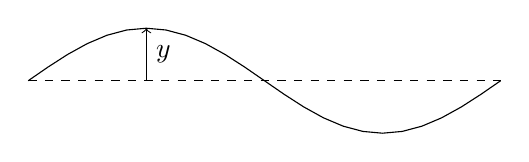
\begin{tikzpicture}
      \draw [domain=0:2] plot ({3*\x}, {sin(\x*180)/1.5});
      \draw [dashed] (0, 0) -- (6, 0);
      \draw [->] (1.5, 0) -- (1.5, 0.666) node [pos = 0.5, right] {$y$};
    \end{tikzpicture}
  \end{center}
  Suppose we pull the line between $x = 0$ and $x = a$ with some tension $T$. Then we set it into motion such that the amplitude is given by $y(x; t)$. Then the kinetic energy is
  \[
    T = \frac{1}{2}\int_0^a \rho v^2\;\d x = \frac{\rho}{2}\int_0^a \dot{y}^2 \;\d x.
  \]
  The potential energy is the tension times the length. So
  \[
    V = T\int \;\d \ell = T\int_0^a\sqrt{1 + (y')^2}\;\d x = (Ta) + \int_0^a \frac{1}{2}T(y'^2)\;\d x.
  \]
  Note that $y'$ is the derivative wrt $x$ while $\dot{y}$ is the derivative wrt time.

  The $Ta$ term can be seen as the \emph{ground-state energy}. It is the energy initially stored if there is no oscillation. Since this constant term doesn't affect where the stationary points lie, we will ignore it. Then the action is given by
  \[
    S[y] = \iint_0^a \left(\frac{1}{2}\rho \dot{y}^2 - \frac{1}{2}T(y')^2\right)\;\d x\;\d t
  \]
  We apply Hamilton's principle which says that we need
  \[
    \delta S[y] = 0.
  \]
  We have
  \[
    \delta S[y] = \iint_0^a \left(\rho \dot{y} \frac{\partial}{\partial t}\delta y - Ty' \frac{\partial}{\partial x}\delta y\right)\;\d x\;\d t.
  \]
  Integrate by parts to obtain
  \[
    \delta S[y] = \iint_0^a \delta y(\rho \ddot{y} - Ty'')\;\d x\;\d t + \text{boundary term}.
  \]
  Assuming that the boundary term vanishes, we will need
  \[
    \ddot{y} - v^2 y'' = 0,
  \]
  where $v^2 = T/\rho$. This is the wave equation in two dimensions. Note that this is a linear PDE, which is a simplification resulting from our assuming the oscillation is small.

  The general solution to the wave equation is
  \[
    y(x, t) = f_+(x - vt) + f_-(x + vt),
  \]
  which is a superposition of a wave travelling rightwards and a wave travelling leftwards.
\end{eg}

\begin{eg}[Maxwell's equations]
  It is possible to obtain Maxwell's equations from an action principle, where we define a Lagrangian for the electromagnetic field. Note that this is the Lagrangian for the \emph{field} itself, and there is a separate Lagrangian for particles moving in a field.

  We have to first define several quantities. First we have the charges: $\rho$ represents the electric charge density and $\mathbf{J}$ represents the electric current density.

  Then we have the potentials: $\phi$ is the electric scalar potential and $\mathbf{A}$ is the magnetic vector potential.

  Finally the fields: $\mathbf{E} = -\nabla \phi - \dot{\mathbf{A}}$ is the electric field, and $\mathbf{B} = \nabla\times \mathbf{A}$ is the magnetic field.

  We pick convenient units where $c = \varepsilon_0 = \mu_0 = 1$. With these concepts in mind, the Lagrangian is given by
  \[
    S[\mathbf{A}, \phi] = \int \left(\frac{1}{2}(|\mathbf{E}|^2 - |\mathbf{B}|^2) + \mathbf{A}\cdot \mathbf{J} - \phi \rho\right)\;\d V\;\d t
  \]
  Varying $\mathbf{A}$ and $\phi$ by $\delta \mathbf{A}$ and $\delta \phi$ respectively, we have
  \[
    \delta S = \int \left(-\mathbf{E}\cdot \left(\nabla \delta\phi + \frac{\partial}{\partial t} \delta \mathbf{A}\right) - \mathbf{B}\cdot \nabla \times \delta \mathbf{A} + \delta \mathbf{A}\cdot \mathbf{J} - \rho\delta\phi\right)\;\d V\;\d t.
  \]
  Integrate by parts to obtain
  \[
    \delta S = \int\left(\delta\mathbf{A}\cdot (\dot{\mathbf{E}} - \nabla\times \mathbf{B} + \mathbf{J}) + \delta \phi(\nabla\cdot \mathbf{E} - \rho)\right)\;\d V\;\d t.
  \]
  Since the coefficients have to be $0$, we must have
  \[
    \nabla \times \mathbf{B} = \mathbf{J} + \dot{\mathbf{E}},\quad \nabla \cdot \mathbf{E} = \rho.
  \]
  Also, the definitions of $\mathbf{E}$ and $\mathbf{B}$ immediately give
  \[
    \nabla\cdot \mathbf{B} = 0,\quad \nabla \times \mathbf{E} = - \dot{\mathbf{B}}.
  \]
  These four equations are Maxwell's equations.
\end{eg}
\section{The second variation}
\subsection{The second variation}
So far, we have only looked at the ``first derivatives'' of functionals. We can identify stationary points, but we don't know if it is a maximum, minimum or a saddle. To distinguish between these, we have to look at the ``second derivatives'', or the \emph{second variation}.

Suppose $x(t) = x_0(t)$ is a solution of
\[
  \frac{\delta F[x]}{\delta y(x)} = 0,
\]
i.e.\ $F[x]$ is stationary at $y = y_0$.

To determine what type of stationary point it is, we need to expand $F[x + \delta x]$ to second order in $\delta x$. For convenience, let $\delta x(t) = \varepsilon \xi(t)$ with constant $\varepsilon \ll 1$. We will also only consider functionals of the form
\[
  F[x] = \int_\alpha^\beta f(x, \dot{x}, t)\;\d t
\]
with fixed-end boundary conditions, i.e.\ $\xi(\alpha) = \xi(\beta) = 0$. We will use both dots ($\dot{x}$) and dashes ($x'$) to denote derivatives.

We consider a variation $x \mapsto x + \delta x$ and expand the integrand to obtain
\begin{align*}
  &f(x + \varepsilon \xi, \dot{x} + \varepsilon \dot{\xi}, t) - f(x, \dot{x}, t)\\
  &= \varepsilon \left(\xi \frac{\partial f}{\partial x} + \dot{\xi}\frac{\partial f}{\partial \dot{x}}\right) + \frac{\varepsilon^2}{2}\left(\xi^2 \frac{\partial^2 f}{\partial x^2} + 2\xi\dot{\xi} \frac{\partial^2 f}{\partial x \partial \dot{x}} + \dot{\xi}^2 \frac{\partial^2 f}{\partial \dot{x}^2}\right) + O(\varepsilon^3)\\
  \intertext{Noting that $2\xi \dot{\xi} = (\xi^2)'$ and integrating by parts, we obtain}
  &= \varepsilon \xi\left[\frac{\partial f}{\partial x} - \frac{\d}{\d t}\left(\frac{\partial f}{\partial \dot{x}}\right)\right] + \frac{\varepsilon^2}{2}\left\{\xi^2\left[\frac{\partial^2 f}{\partial x^2} - \frac{\d}{\d t}\left(\frac{\partial^2 f}{\partial x\partial \dot{x}}\right)\right] + \dot{\xi}^2 \frac{\partial f}{\partial \dot{x}^2}\right\}.
\end{align*}
plus some boundary terms which vanish. So
\[
  F[x + \varepsilon \xi] - F[x] = \int_\alpha^\beta\varepsilon\xi\left[\frac{\partial f}{\partial x} - \frac{\d}{\d t}\left(\frac{\partial f}{\partial \dot{x}}\right)\right]\;\d t + \frac{\varepsilon^2}{2}\delta^2 F[x, \xi] + O(\varepsilon^3),
\]
where
\[
  \delta^2 F[x, \xi] = \int_\alpha^\beta \left\{\xi^2 \left[\frac{\partial^2 f}{\partial x^2} - \frac{\d}{\d t}\left(\frac{\partial^2 f}{\partial x \partial \dot{x}}\right)\right] + \dot{\xi}^2 \frac{\partial^2 f}{\partial \dot{x}^2}\right\}\;\d t
\]
is a functional of both $x(t)$ and $\xi(t)$. This is analogous to the term
\[
  \delta \mathbf{x}^T H(\mathbf{x})\delta \mathbf{x}
\]
appearing in the expansion of a regular function $f(\mathbf{x})$. In the case of normal functions, if $H(\mathbf{x})$ is positive, $f(\mathbf{x})$ is convex for all $\mathbf{x}$, and the stationary point is hence a global minimum. A similar result holds for functionals.

In this case, if $\delta^2 F[x, \xi] > 0$ for all non-zero $\xi$ and all allowed $x$, then a solution $x_0(t)$ of $\frac{\delta F}{\delta x} = 0$ is an absolute minimum.

\begin{eg}[Geodesics in the plane]
  We previously shown that a straight line is a stationary point for the curve-length functional, but we didn't show it is in fact the shortest distance! Maybe it is a maximum, and we can get the shortest distance by routing to the moon and back.

  Recall that $f = \sqrt{1 + (y')^2}$. Then
  \[
    \frac{\partial f}{\partial y} = 0,\quad \frac{\partial f}{\partial y'} = \frac{y'}{\sqrt{1 + (y')^2}},\quad \frac{\partial^2 f}{\partial y'^2} = \frac{1}{\sqrt{1 + (y')^2}^3},
  \]
  with the other second derivatives zero. So we have
  \[
    \delta ^2 F[y, \xi] = \int_\alpha^\beta \frac{\dot{\xi}^2}{(1 + (y')^2)^{3/2}}\;\d x > 0
  \]
  So if we have a stationary function satisfying the boundary conditions, it is an absolute minimum. Since the straight line is a stationary function, it is indeed the minimum.
\end{eg}
However, not all functions are convex\textsuperscript{[\textcolor{blue}{citation needed}]}. We can still ask whether a solution $x_0(t)$ of the Euler-Lagrange equation is a local minimum. For these, we need to consider
\[
  \delta^2 F[x_0, \xi] = \int_\alpha^\beta (\rho(t)\dot{\xi}^2 + \sigma(t) \xi^2)\;\d t,
\]
where
\[
  \rho(t) = \left.\frac{\partial^2 f}{\partial \dot{x}^2}\right|_{x = x_0},\quad
  \sigma(t) = \left[\frac{\partial^2 f}{\partial x^2} - \frac{\d}{\d t}\left(\frac{\partial^2 f}{\partial x \partial \dot{x}}\right)\right]_{x = x_0}.
\]
This is of the same form as the Sturm-Liouville problem. For $x_0$ to minimize $F[x]$ locally, we need $\delta^2 F[x_0, \xi] > 0$. A necessary condition for this is
\[
  \rho(t) \geq 0,
\]
which is the \emph{Legendre condition}.

The intuition behind this necessary condition is as follows: suppose that $\rho(t)$ is negative in some interval $I\subseteq [\alpha, \beta]$. Then we can find a $\xi(t)$ that makes $\delta^2 F[x_0, \xi]$ negative. We simply have to make $\xi$ zero outside $I$, and small but crazily oscillating inside $I$. Then inside $I$, $\dot{x}^2$ wiill be very large while $\xi^2$ is kept tiny. So we can make $\delta^2 F[y, \xi]$ arbitrarily negative.

Turning the intuition into a formal proof is not difficult but is tedious and will be omitted.

However, this is not a sufficient condition. Even if we had a strict inequality $\rho (t) > 0$ for all $\alpha < t < \beta$, it is still not sufficient.

Of course, a sufficient (but not necessary) condition is $\rho(t) > 0, \sigma(t) \geq 0$, but this is not too interesting.

\begin{eg}
  In the Branchistochrone problem, we have
  \[
    T[x] \propto \int_\alpha^\beta \sqrt{\frac{1 + \dot{x}^2}{x}}\;\d t.
  \]
  Then
  \begin{align*}
    \rho(t) &= \left.\frac{\partial^2 f}{\partial \dot{x}^2}\right|_{x_0} > 0\\
    \sigma(t) &= \frac{1}{2x^2\sqrt{x(1 + \dot{x}^2)}} > 0.
  \end{align*}
  So the cycloid does minimize the time $T$.
\end{eg}
\subsection{Jacobi condition for local minima of \texorpdfstring{$F[x]$}{F[x]}}
Legendre tried to prove that $\rho > 0$ is a sufficient condition for $\delta^2 F > 0$. This is known as the \emph{strong Legendre condition}. However, he obviously failed, since it is indeed not a sufficient condition. Yet, it turns out that he was close.

Before we get to the actual sufficient condition, we first try to understand why thinking $\rho > 0$ is sufficient isn't as crazy as it first sounds.

If $\rho > 0$ and $\sigma < 0$, we would want to create a negative $\delta^2 F[x_0, \xi]$ by choosing $\xi$ to be large but slowly varying. Then we will have a very negative $\sigma(t)\xi^2$ while a small positive $\rho(t) \dot{\xi^2}$.

The problem is that $\xi$ has to be $0$ at the end points $\alpha$ and $\beta$. For $\xi$ to take a large value, it must reach the value from $0$, and this requires some variation of $\xi$, thereby inducing some $\dot{\xi}$. This is not a problem if $\alpha$ and $\beta$ are far apart - we simply slowly climb up to a large value of $\xi$ and then slowly rappel back down, maintaining a low $\dot{\xi}$ throughout the process. However, it is not unreasonable to assume that as we make the distance $\beta - \alpha$ smaller and smaller, eventually all $\xi$ will lead to a positive $\delta^2 F[x_0, \xi]$, since we cannot reach large values of $\xi$ without having large $\dot{\xi}$.

It turns out that the intuition is correct. As long as $\alpha$ and $\beta$ are sufficiently close, $\delta^2 F[x_0, \xi]$ will be positive. The derivation of this result is, however, rather roundabout, involving a number of algebraic tricks.

For a solution $x_0$ to the Euler Lagrange equation, we have
\[
  \delta^2 F[x_0, \xi] = \int_\alpha^\beta \big(\rho(t) \dot{\xi}^2 + \sigma(t) \xi^2\big)\;\d t,
\]
where
\[
  \rho(t) = \left.\frac{\partial^2 f}{\partial \dot{x}^2}\right|_{x = x_0},\quad
  \sigma(t) = \left[\frac{\partial^2 f}{\partial x^2} - \frac{\d}{\d t}\left(\frac{\partial^2 f}{\partial x \partial \dot{x}}\right)\right]_{x = x_0}.
\]
Assume $\rho(t) > 0$ for $\alpha < t < \beta$ (the strong Legendre condition) and assume boundary conditions $\xi(\alpha) = \xi(\beta) = 0$. When is this sufficient for $\delta^2 F > 0$?

First of all, notice that for any smooth function $w(x)$, we have
\[
  0 = \int_\alpha^\beta (w\xi^2)' \;\d t
\]
since this is a total derivative and evaluates to $w\xi(\alpha) - w\xi(\beta) = 0$. So we have
\[
  0 = \int_\alpha^\beta (2w\xi \dot{\xi} + \dot{w}\xi^2)\;\d t.
\]
This allows us to rewrite $\delta^2 F$ as
\[
  \delta^2 F = \int_\alpha^\beta \big(\rho \dot{\xi}^2 + 2w\xi \dot{\xi} + (\sigma + \dot{w})\xi^2\big)\;\d t.
\]
Now complete the square in $\xi$ and $\dot{\xi}$. So
\[
  \delta^2 F = \int_\alpha^\beta \left[\rho\left(\dot{\xi} + \frac{w}{\rho} \xi\right)^2 +\left(\sigma + \dot{w} - \frac{w^2}{\rho}\right)\xi^2 \right]\;\d t
\]
This is non-negative if
\[
  w^2 = \rho(\sigma + \dot{w}).\tag{$*$}
\]
So as long as we can find a solution to this equation, we know that $\delta^2 F$ is non-negative. Could it be that $\delta^2 F = 0$? Turns out not. If it were, then $\dot{\xi} = -\frac{w}{\rho}\xi$. We can solve this to obtain
\[
  \xi(x) = C\exp\left(-\int_\alpha^x \frac{w(s)}{\rho(s)}\;\d s\right).
\]
We know that $\xi(\alpha) = 0$. But $\xi(\alpha) = C e^0$. So $C = 0$. Hence equality holds only for $\xi = 0$.

So all we need to do is to find a solution to $(*)$, and we are sure that $\delta^2 F > 0$.

Note that this is non-linear in $w$. We can convert this into a linear equation by defining $w$ in terms of a new function $u$ by $w = -\rho \dot{u}/u$. Then $(*)$ becomes
\[
  \rho\left(\frac{\dot{u}}{u}\right)^2 = \sigma - \left(\frac{\rho \dot{u}}{u}\right)' = \sigma - \frac{(\rho \dot{u})'}{u} + \rho \left(\frac{\dot{u}}{u}\right)^2.
\]
We see that the left and right terms cancel. So we have
\[
  -(\rho \dot{u})' + \sigma u = 0.
\]
This is the \emph{Jacobi accessory equation}, a second-order linear ODE.

There is a caveat here. Not every solution $u$ will do. Recall that $u$ is used to produce $w$ via $w = -\rho\dot{u}/u$. Hence within $[\alpha, \beta]$, we cannot have $u = 0$ since we cannot divide by zero. If we can find a non-zero $u(x)$ satisfying the Jacobi accessory equation, then $\delta^2 F > 0$ for $\xi \not= 0$, and hence $y_0$ is a local minimum of $F$.

A suitable solution will always exists for sufficiently small $\beta - \alpha$, but may not exist if $\beta - \alpha$ is too large, as stated at the beginning of the chapter.

\begin{eg}[Geodesics on unit sphere]
  For any curve $C$ on the sphere, we have
  \[
    L = \int_C \sqrt{\d \theta^2 + \sin^2 \theta \;\d \phi^2}.
  \]
  If $\theta$ is a good parameter of the curve, then
  \[
    L[\phi] = \int_{\theta _1}^{\theta_2} \sqrt{1 + \sin^2 \theta (\phi')^2}\;\d \theta.
  \]
  Alternatively, if $\phi$ is a good parameter, we have
  \[
    L[\theta] = \int_{\phi_1}^{\phi_2}\sqrt{(\theta')^2 + \sin^2 \theta}\;\d \phi.
  \]
  We will look at the second case.

  We have
  \[
    f(\theta, \theta') = \sqrt{(\theta')^2 + \sin^2 \theta}.
  \]
  So
  \[
    \frac{\partial f}{\partial \theta} = \frac{\sin \theta\cos \theta}{\sqrt{(\theta')^2 + \sin^2 \theta}},\quad \frac{\partial f}{\partial \theta'} = \frac{\theta'}{\sqrt{(\theta')^2 + \sin^2 \theta}}.
  \]
  Since $\frac{\partial f}{\partial \phi} = 0$, we have the first integral
  \[
    \text{const} = f - \theta' \frac{\partial f}{\partial \theta'} = \frac{\sin^2 \theta}{\sqrt{(\theta')^2 + \sin^2 \theta}}
  \]
  So a solution is
  \[
    c\sin^2 \theta = \sqrt{(\theta')^2 + \sin^2 \theta}.
  \]
  Here we need $c \geq 1$ for the equation to make sense.

  We will consider the case where $c = 1$ (in fact, we can show that we can always orient our axes such that $c = 1$). This occurs when $\theta' = 0$, i.e.\ $\theta$ is a constant. Then our first integral gives $\sin^2 \theta = \sin \theta$. So $\sin \theta = 1$ and $\theta = \pi/2$. This corresponds to a curve on the equator. (we ignore the case $\sin \theta = 0$ that gives $\theta = 0$, which is a rather silly solution)

  There are two equatorial solutions to the Euler-Lagrange equations. Which, if any, minimizes $L[\theta]$?
  \begin{center}
    \begin{tikzpicture}
      \draw circle [radius=2];
      \draw [red] (2, 0) arc (0:240:2 and 0.5);
      \draw [red] (2, 0) arc (0:-60:2 and 0.5);
      \draw [blue] (0, -0.5) arc (-90:-60:2 and 0.5) node [circ] {};
      \draw [blue] (0, -0.5) arc (270:240:2 and 0.5) node [circ] {};
    \end{tikzpicture}
  \end{center}
  We have
  \[
    \left.\frac{\partial^2 f}{\partial (\theta')^2}\right|_{\theta = \pi/2} = 1
  \]
  and
  \[
    \frac{\partial^2 f}{\partial \theta \partial \theta'} = -1,\quad \frac{\partial^2}{\partial \theta\partial \theta'} = 0.
  \]
  So $\rho(x) = 1$ and $\sigma(x) = -1$. So
  \[
    \delta^2 F = \int_{\phi_1}^{\phi_2} ((\xi')^2 - \xi^2)\;\d \phi.
  \]
  The Jacobi accessory equation is $u'' + u = 0$. So the general solution is $u \propto \sin \phi - \gamma \cos\phi$. This is equal to zero if $\tan \phi = \gamma$.

  Looking at the graph of $\tan \phi$, we see that $\tan$ has a zero every $\pi$ radians. Hence if the domain $\phi_2 - \phi_1$ is greater than $\pi$ (i.e.\ we go the long way from the first point to the second), it will always contain some values for which $\tan \phi$ is zero. So we cannot conclude that the longer path is a local minimum (it is obviously not a global minimum, by definition of longer) (we also cannot conclude that it is \emph{not} a local minimum, since we tested with a sufficient and not necessary condition). On the other hand, if $\phi_2 - \phi_1$ is less than $\pi$, then we will be able to pick a $\gamma$ such that $u$ is non-zero in the domain.
\end{eg}
\end{document}

